\chapter{インターネットプロトコル層(その2) アドレスとルーティング}

概論に続いて、今度はインターネットプロトコル層に踏み込んでいくことにしましょう。どのような方法でパケットによる通信を行っているのか、そして、どのようにパケットが通信相手に届くのか。それを説明します。


\section{IPアドレス}

IPアドレスは、どのネットワークであるかを表すネットワークアドレス部分と、ネットワークの中でホストを特定するホストアドレス部分とに分けることができる。このことは、IPv4もIPv6も相違はない。それを論じるために、本章で用いる「ネットワーク」という用語について定義を行おう。
本章で注釈なくネットワークという言葉を使用した場合は、独立して存在するネットワーク、つまりネットワークコミュニケーション層を指すものとする。

\subsection{IPアドレスの構造}

IPアドレスにおけるネットワークアドレス部分とは、どのネットワークであるかを判別するための部分である。住所でたとえれば、ビル名までに相当すると考えればよいだろう。ネットワークアドレス部分を見ることで、どのネットワークであるか、つまり、どこの住所に建っているビルかがわかるわけだ。

IPアドレスのホストアドレス部分とは、ネットワークアドレス部分で特定されたネットワークの中で、どのホストかを特定するアドレスである。先の住所のたとえで表せば、ビルの部屋番号と考えればよいだろう。

今度は郵便配達にたとえてみよう。郵便配達では、通常はビル名までの住所(ネットワークアドレス)によって、郵便物が届けられる。そして、そのビルに郵便物を代表して受け取る仕組み(ルータ)があったとしたら、ビル(ネットワーク)内で部屋番号(ホストアドレス)による配達は、代表して受け取った者(ルータ)の仕事、ということである。

\subsection{ネットワークアドレス}

IPアドレスは、ネットワークアドレスとホストアドレスに分かれる。では、先程の例えでは建物名までに相当するネットワークアドレスは、どのように表せば良いのだろうか。住所で部屋番号を省略した場合、建物名となる。それと同じである。

IPアドレスの用語で言えば、ホストアドレスを省略すれば、それはネットワークのアドレスとなる。ホストアドレスの省略とは、ホストアドレス部のビットを全て0にすることである。
IPv4でもIPv6でも、ホストアドレス部分のビットを全て0にした場合、それはネットワークそのものをあらわすIPアドレスとして用いられる。

\subsection{IPv4アドレスの構造}

\begin{figure}[htbp]
	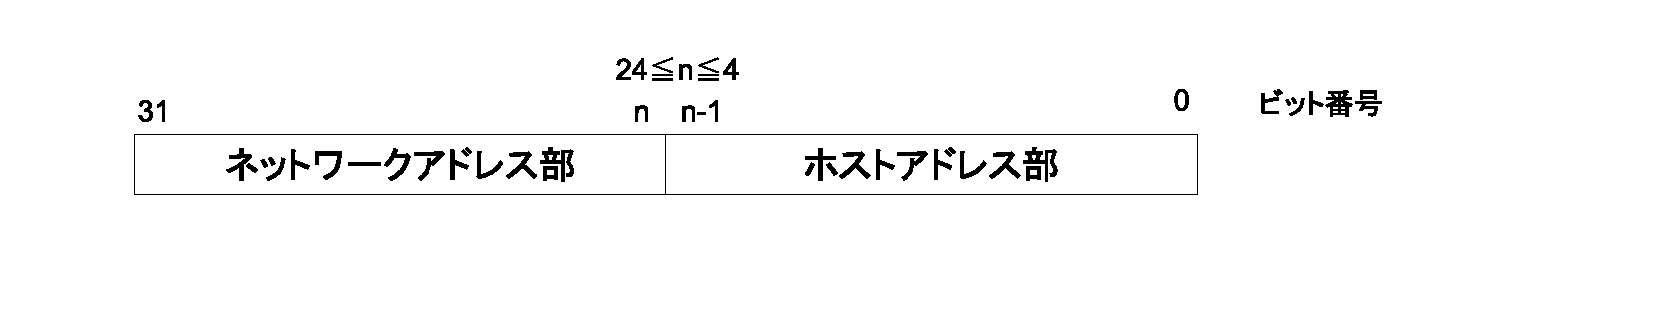
\includegraphics[width=12cm,clip]{draw/ipaddr.eps}
	\caption{IPv4アドレスの構造}
	\label{fig:ipaddr}
\end{figure}

IPアドレスは、ネットワークアドレス部とホストアドレス部に分けられる。では、IPアドレスの中で、ネットワークアドレスとホストアドレスをどのように区別するのか。

IPv4のネットワークアドレス部は、IPアドレスを32bitのビット列と見たときに、先頭から8ビット以上連続するビット列である。また、ホストアドレス部はその残りである。つまり、IPアドレスとは、ネットワークアドレス部のビット列と、ホストアドレス部のビット列を連結したものと考えることができる。つまり、ネットワークアドレス部とホストアドレス部の間には、なんらかの区切りがある。

では、32ビットのIPアドレスの中で、ネットワークアドレスとホストアドレスはどのように区別するかを改めて考えよう。それには、ビット列の先頭から何ビット目までをネットワークアドレスと見なし、それ以降のビットをホストアドレスと見なす、という区切りを記載すればよいのではないだろうか。
その区切りは先頭から8bit目以降30ビットまでの任意\footnote{実際には割り当てを受けるので好き勝手に付けていいわけではない}のビット数をネットワークアドレス、残りをホストアドレスとして使用する。

このように、ネットワークアドレスとホストアドレスの境目が8ビット目以降30ビット目までのどこかになる、という分割方法を、クラスレス、もしくはCIDR(Classless Inter-Domain Routing)と呼ぶ。

\subsection{IPv4アドレスの表記}
IPv4アドレスは、32bitの長さを持っている。これを、先頭から8bitごとに区切って10進数で表記する。区切りにはドットを用いる。例えば、00001010000011110000000000000001というiPv4アドレスがあるとしよう。

まず先頭から8bitごとに区切って00001010.00001111.00000000.00000001である。これを区切りごとに8bitの値とみて10進数で書くと、10.15.0.1となる。

\subsection{IPv4のクラスフルとクラスレス}

かつては、ネットワークアドレスとホストアドレスの区切りは、8ビット、16ビット、24ビットの三種類であった。これを、クラスフル、もしくはナチュラルクラスと呼んでいた。 IPアドレスを記述するときに8ビットごとに十進数にしてドットで区切ってならべるというのは、この時代の名残である。また、区切りが8ビット目のネットワークアドレスをクラスA,16ビット目のネットワークアドレスをクラスB,24ビット目のネットワークアドレスをクラスCと呼んでいた。

クラスとホストアドレス数の関係をまとめると、表\ref{ipclass}のようになる。

\begin{table}[hbtp] \caption{IPアドレスのクラス} \label{ipclass}
\begin{center}
\begin{tabularx}{110mm}{XXX} \toprule
クラス & ネットワークアドレスの区切り & ホストアドレス個数\\ \midrule
クラスA & 8bit目 & 16Mi個\\
クラスB & 16bit目 & 65535個\\
クラスC & 24bit目 & 255個\\ \bottomrule
\end{tabularx}
\end{center}
\end{table}

グローバルなIPアドレスの割り当ては、この8ビット毎の区切りで、その組織に必要なIPアドレスの数に最も近いクラスで行われていた。そのため、 2001年くらいまでは、社員が10人もいない会社がクラスCのグローバルアドレスをもらうのも珍しくなかった\footnote{ネットワークプリンタにグローバルIPアドレスが割り当てられるような使い方をしているところも珍しくなかった}。また、学術機関でも、MITは以前クラスAを割り当てられていたし、国内の大学でjunetやWIDEの頃からインターネット接続をしているところでは、クラスBの割り当ても珍しくなかった。

\subsection{クラスDとクラスE}
クラスフルの解説を行うと、クラスDやクラスEというものがあらわれる。だが、これらはここまで解説したような、グローバルなIPアドレスに対して、ネットワークアドレスとホストアドレスの区切りを表すものではない

クラスDは、IPマルチキャストという、インターネットプロトコルにおけるマルチキャストを行う場合に使用するために予約されている領域である。クラスDのアドレスは、アドレス毎に意味が設定されている。そのため、ネットワークアドレス、ホストアドレスの区別はない。\footnote{クラスDアドレスの意味は、IANAで規定されている。詳細はhttp://www.iana.org/assignments/multicast-addressesを参照されたい。}

クラスEは、予約領域とされている。そのため、実際のネットワークには割り当てられない。

\subsection*{}
\begin{itembox}[l]{いもうとコラム IPv4クラスフルアドレスのネットワークアドレス部分判別}

IPv4をクラスフルで使っていた頃は、少なくとも、ネットワークアドレスとホストアドレスの区切りの位置を、どのように判別していたのでしょうか。
IPv4アドレスは、クラス毎にネットワークアドレスの先頭の数ビットのパターンが決められていました。つまり、IPアドレスの先頭のビットパターンを見ることで、どのクラスのアドレスかわかります。

そのため、インターネットプロトコルの中には、ネットマスクを伝達する機能がありません。このことは、IPv4がクラスフルからクラスレスになったときに恩恵と問題をもたらしました。それについてはまた後ほど解説することにします。
クラスの区別をするための、IPアドレス先頭のビットパターンは表\ref{bitpattern}です。

クラスレスのIPアドレスが使用されている現在でも、ネットワークアドレス部分が8ビット以上必要であるのは、クラスフルのIPアドレスとの互換性維持のためです。


\end{itembox}

\begin{table}[hbtp] \caption{クラス別のネットワークアドレスのビットパターン} \label{bitpattern}
\begin{center}
\begin{tabularx}{110mm}{lll} \toprule
クラス & ネットワークアドレスのビットパターン & 取りうるIPアドレスの範囲\\ \midrule
A & 0xxxxxxx & $0.0.0.0-127.255.255.255$\\
B & 10xxxxxx\_ xxxxxxxx & $128.0.0.0-191.255.255.255$\\
C & 110xxxxx\_ xxxxxxxx\_ xxxxxxxx & $192.0.0.0-223.255.255.255$\\
D & 1110xxxx\_ xxxxxxxx\_ xxxxxxxx & $224.0.0.0-239.255.255.255$\\
E & 1111xxxx\_ xxxxxxxx\_ xxxxxxxx & $240.0.0.0-255.255.255.255$\\ \bottomrule
\end{tabularx}
\end{center}
\end{table}


\subsection{ネットマスク記法}

では、IPv4アドレスの、ネットワークアドレスとホストアドレスの区切りは、どのように表現するののだろうか。それをあらわすために、まずはIPv4のクラスレスアドレスの場合を説明しよう。

クラスレスのネットワークアドレスとホストアドレスの区別をつけるためには、ネットマスクというものを用いる。

ネットマスクは、IPアドレスと同じビット列で、IPアドレスと同様に、IPv4であれば、8ビットごとにドットで区切って、区切りことに10進数で表記する。そして、ネットワークアドレスとホストアドレスの区切りをあらわしたいIPアドレスの、ネットワークアドレスのビット数と同じビット数、先頭から1が続き、残りのビットが0になる。

たとえば、先頭から24ビットまでがネットワークアドレスであるIPv4アドレスでは、ビットマスクは$11111111.11111111.11111111.00000000$となる。十進数で記述すれば$255.255.255.0$となるわけだ。

ではこのビット列をネットマスクと呼ぶのはなぜだろうか。それは、IPアドレスとネットマスクの間で論理演算を行うと、ネットワークアドレスを取り出すことができるからである。IPアドレスとネットマスクの間でAND(論理積)をとると、ネットワークアドレス部分のビット列はそのまま残り、ホストアドレス部分のビット列はすべて0になる。その演算結果は、ネットワークアドレスである。
ネットマスクをIPアドレスに併記する場合は、$192.168.0.1/255.255.255.0$というように、IPアドレスの後をスラッシュで区切り、その後にネットマスクを記載する。

ここで気をつけるのは、ネットマスクは、かならず先頭から1のビットが連続し、残りのビットがすべて0という構造となるということだ。たとえば、$255.255.255.128$というネットマスクは存在する。これは、先頭から25ビット1が連続する、$11111111.11111111.11111111.10000000$というネットマスクであるからである。だが、たとえば、$255.255.255.129$という、2進数で記述すると$11111111.11111111.11111111.10000001$となるネットマスクは存在しない。


\subsection{プレフィックス長}

ここまで、$255.255.255.0$のように記述してきたIPv4ネットマスクだが、省略した記法がある。

ネットマスクを併記すると、IPアドレスの記述が長くなる。そこで、プレフィックス長という省略記法がある。

ネットマスクは、、先頭から必ず1が連続するビット列である。そこで、連続した1の数をネットマスクとして書けばよい。IPアドレスの後にスラッシュをつけ、その後にネットマスクの先頭から何ビット目まで1かの数字を記載するのが、プレフィックス長の記法である。。

ネットマスク$255.255.255.0$であれば、ビット列は$11111111.11111111.11111111.00000000$となり、1は先頭から数えて24ビット連続する。そこで、このネットマスクを、/24と記載する。192.168.1.1/24であれば、ネットワークアドレス192.168.1で、ネットマスクは$255.255.255.0$となる。

\subsection{IPv4ネットワークアドレスの省略記法}
IPv4のネットワークアドレスを十進数で記述する際に、末尾から、ドット区切りの
0が連続するときは、それを省略して記述することがある。
たとえば、192.168/24という記述をしている場合、それは、192.168.0.0/24というネットワークアドレスを表す。

この省略記法で注意するのは、ネットワークアドレスの末尾に、十進数で表した場合の0が連続するときのみ省略可能ということである。つまり、省略可能なのは、ネットワークアドレスが8ビット、16ビット、24ビットのいずれかで、ネットワークアドレスの末尾が0である場合のみである。



\subsection{IPv4アドレスの範囲の表現}
IPv4で、ネットマスクは、IPアドレスの範囲を表すためにも用いられる。たとえば、IPアドレスを、192.168.1.16から連続する16個指定したいとしよう。16個のIPアドレスを記載すると、煩雑であり、タイプミスも生じるであろう。

そのため、ネットマスクは、アプリケーションでIPアドレスを設定する際など、IPアドレスの範囲を表したい場合にも用いられる。その範囲において、IPアドレスのビット列が共通となる部分にマスクをかけるわけだ。ここでネットマスクを掛けるのは、IPアドレスのビット列の共通部分であって、ネットワークアドレスの範囲でないことに気をつけたい。
あるネットマスクが、ネットワークアドレスを表すためのものか、IPアドレスの範囲をあらわすものかは、それがあらわれた文脈で判断する必要があ。

192.168.1.16から連続する16個のIPアドレスは、先頭28ビットまでのビット列が共通である。そのため、その範囲を表すには192.168.1.16/255.255.255.240もしくは192.168.1.16/28と記述する。

IPアドレスの範囲を表す記法において、255.255.255.255もしくは/32というネットマスクが用いられることがある。この場合、そのIPアドレスただ一つが範囲であるという意味になる。
逆に、IPアドレスの範囲を表す際に、特に、全てのIPアドレスであることを表したい場合は、/0.0.0.0もしくは/0として表すこともある。だがこの場合、IPアドレスの方も0.0.0.0として、0.0.0.0/0と表すことが多い。

IPアドレスの範囲をネットマスクで表す場合、表せる範囲とは、ネットマスクのビット列で共通範囲を表せるものとなる。これがどういうことかというと、2進数できりのいい数の範囲でしか表すことができないということだ。
たとえば、192.168.1.0から192.168.1.127までのIPアドレスの範囲は、共通部分をネットワークアドレスと見た場合のネットマスクは/25であり、IPアドレスの範囲はイコール、残り7ビットで表されるホストアドレスの範囲となる。つまり、このIPアドレスの範囲は192.168.1.0/25として表すことができる。だが、192.168.1.0から192.168.1.100までというIPアドレスの範囲は、ホストアドレスの範囲が、7ビットで表されるホストアドレスの範囲と一致しない。そのため、先頭からの連続するビットで共通部分を抜き出すことができない。つまり、ネットマスク記法で範囲を記述することができない。

\subsection{IPv6アドレスの構造}

\begin{figure}[htbp]
	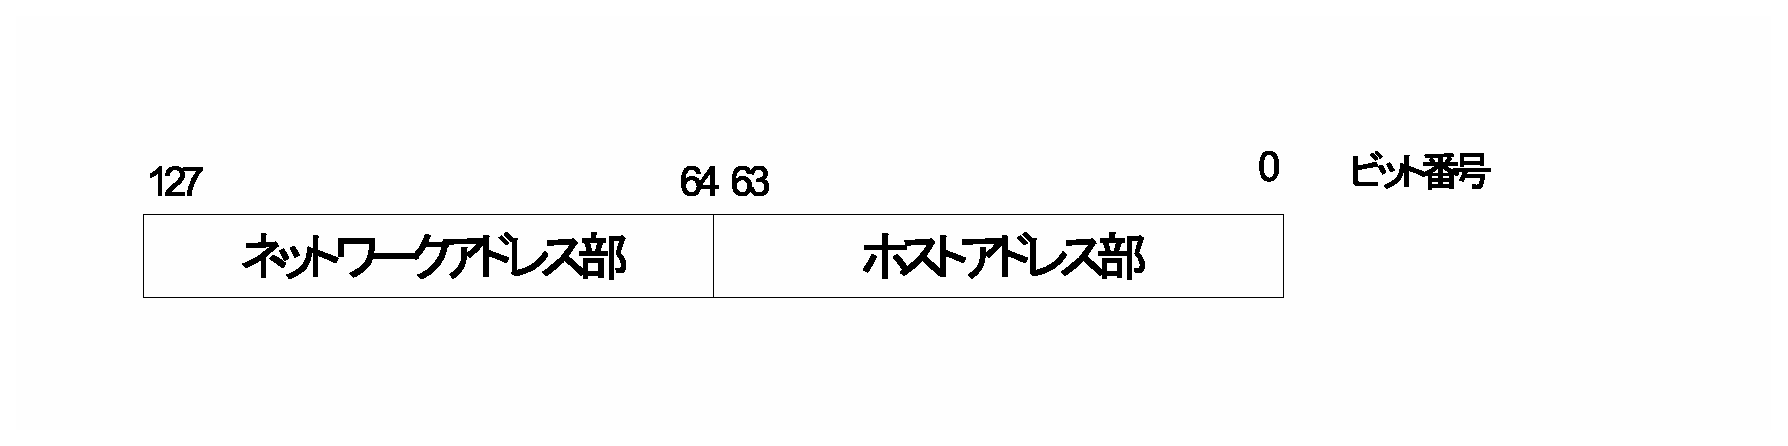
\includegraphics[width=12cm,clip]{draw/ip6addr.eps}
	\caption{IPv6アドレスの構造}
	\label{fig:ipaddr}
\end{figure}


IPv6では、ネットワークアドレスとホストアドレスの区切りは、1ビット単位で設定することができる。だが、IPv6の機能である、IPv6アドレスの自動割り当て機能を利用しようとする場合、ネットワークアドレス64bit、ホストアドレス64bitであることがRFC4291によって求められている。
そのため、一般的なネットワーク設定では、先頭64bitをネットワークアドレスとして扱い、残り64bitをホストアドレスとして設定する。この理由から、実用上は64bitで区切られる、と考えて良いだろう。

\subsection{IPv6アドレスの表記}
IPv6のアドレスは、128bit長ある。仮にIPv4と同じやり方で表記したとすると、16組の10進数の数字が並ぶことになる。そこで、IPv6では、ビット列を16bitごとに区切り、それぞれを16進数で表記する。つまり、16進数4桁が8組並んだものが、IPv6のアドレスとなる。
この4桁の16進数8組を、コロンで連結してひとつのアドレスとする。

0と1が128個並ぶことになるのででビット列は省略するが、たとえば、2001:0db8:0000:0000:0001:0000:0000:0123というように、IPv6アドレスはあらわされる。


\subsection{IPv6のプレフィクス長}
IPv6では、ネットワークアドレスとホストアドレスの区切りを示すのに、ネットマスク表記ではなくプレフィクス長を用いる。IPv6の場合は128bitの長さがあるため、IPv5のようなネットマスク表記をすれば、FFFF:FFFF:FFFF:FFFF:00000:0000:0000:0000というように、とても長くなってしまうためだ。この場合、プレフィクス長を用いて/64と表現する。

IPv6のアドレスは、128bitである。そのため、プレフィクス長は最大で/128ということににある。
IPv4と同様に、ビット長である/128を用いるときは、ネットワークアドレスの範囲でなく、そのIPアドレスただ一つであることをあらわす。


\subsection{IPv6アドレスの省略記法}
IPv6アドレスは、きちんと書くと長い。そのため、少しでも短く記述するための省略記法が設定されている。その省略は、以下のルールで行わうことが許されている。

\paragraph{16bitごとの先頭の0は省略できる}
16bit区切りごとの、先頭の0は省略することができる。たとえば、IPアドレスの先頭が32bitが2001:0db8:であるとすれば、2001:db8:というように、0db8の先頭の0省略して記述することができる。

\paragraph{連続する0は一箇所だけ省略できる}
16bitの区切りで、0000と表現される部分があれば、一箇所だけ表記そのものを省略してかまわない。また、それが連続して現れれば、まとめて省略することができる。2001:0db8:0000:0000:0000:0000:0000:0123であれば、2001:db8::123というように表記する。その省略部分は::と、コロン二つで記述する。

この省略規則では、一箇所以上の連続があった場合は、そのうちの一箇所だけを省略可能となる。た先に例として用いた、、2001:0db8:0000:0000:0001:0000:0000:0123というアドレスを省略する場合で考えてみよう・、

2001:db8::1::0000:0000:123と書くか、2001:db8:0000:0000:1::123と書くか、どちらにでも表記することができる。だが、2001:db8::1::123という表記をすると、省略部分に挟まれた0001が、128bitのどこにはいるかわからなくなってしまう。

この省略記法を用いいる場合、128ビット全てが0のアドレスは::、一番最後のビットだけ1のアドレスは::1と表記することができる。詳しくは後述するが、それぞれ、デフォルトルートをあらわすアドレスと、ループバックアドレスに付けるアドレスである。

\subsection{IPアドレスの分類}

IPアドレスには、どのような宛先を表すかでいくつかの種類がある。ユニキャスト、マルチキャスト、ブロードキャスト、そして、IPv6で追加された概念として、エニーキャストである。それぞれについて説明をしていく。

\subsubsection{ユニキャストアドレス}

\begin{figure}[htbp]
	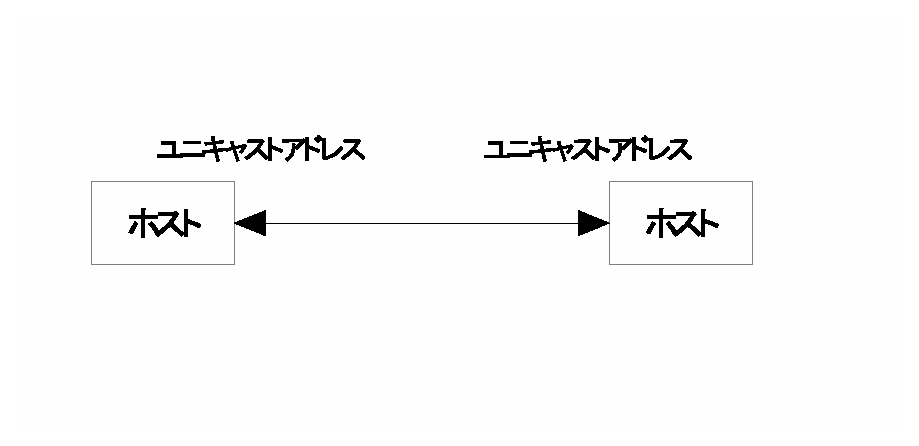
\includegraphics[width=12cm,clip]{draw/unicast.eps}
	\caption{ユニキャストアドレス}
	\label{fig:unicast}
\end{figure}

ユニキャストアドレスは、あるネットワークの範囲で、たった一つのネットワークインタフェイスを表すためのアドレスである。あるユニキャストアドレス当てに送信されたパケットは、そのアドレスに定められたネットワークの範囲において、ただ一つのネットワークインタフェイスに到達する。つまり、ただ一つのホストを宛先としたい場合に、ユニキャストアドレスを使用する。

IPv4、IPv6の両方に、ユニキャストアドレスの概念がある。


\subsubsection{マルチキャストアドレス}
\begin{figure}[htbp]
	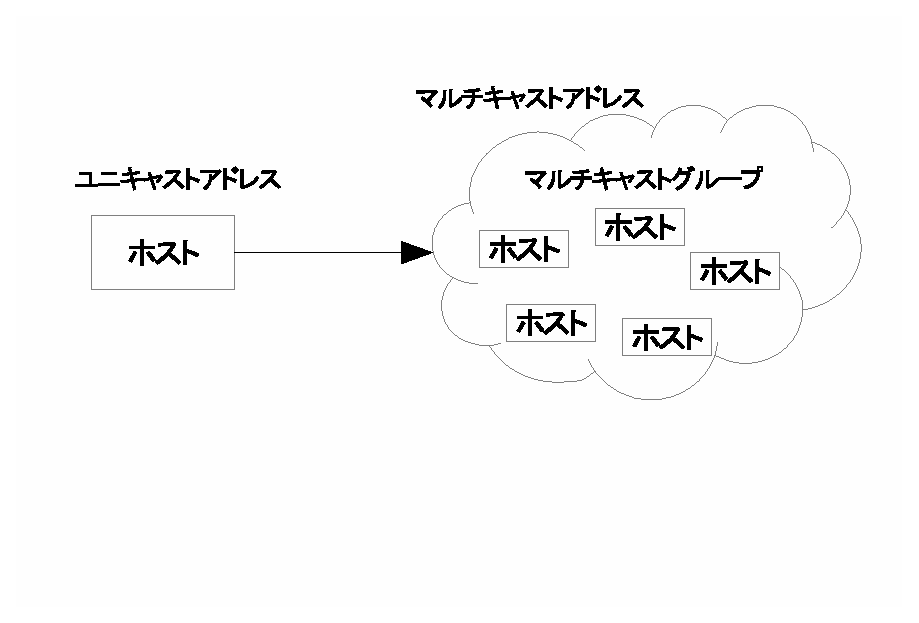
\includegraphics[width=12cm,clip]{draw/multicast.eps}
	\caption{マルチキャストアドレス}
	\label{fig:multicast}
\end{figure}

マルチキャストアドレスは、あるネットワークの範囲で、ネットワークのインタフェイスのグループを表すアドレスである。あるマルチキャストアドレス宛に送ったデータグラムは、同じマルチキャストアドレスを持つネットワークインタフェイス全てに到着する。あるグループに属する全てのホストに対して、同じデータを送信したい場合にマルチキャストアドレスを指定する。

マルチキャストアドレスは、その性質から、トランスポート層のプロトコルで、TCPのようなコネクション指向のものを使用することはできない。

マルチキャストは、IPv4では後で拡張された概念である。一方、IPv6では最初から導入されており、インターネットプロトコル層での制御に用いられる。

\subsubsection{ブロードキャストアドレス}
IPv4で、同じネットワーク内の全てのホストを表すアドレスである。ブロードキャスト宛ての通信は、そのネットワークの中の全てのホストが受信する。そのため、放送(ブロードキャスト)アドレスと呼ぶわけだ。

IPv4では、ホストアドレス部分のビットを全て1にすると、ブロードキャストアドレスとなる。たとえば、192.168.1.0/24というネットワークのブロードキャストアドレスは、ホストアドレス部分である下位8bitをすべて1にした192.168.1.255となる。

IPv6には、ブロードキャストアドレスはない。ではどのようにしているのだろうか。IPv6では、ブロードキャストに相当する宛先を利用したい場合は、「全てのホスト宛のマルチキャストアドレス」を使用する。そのため、IPv6にはブロードキャストはない。

\subsubsection{エニーキャストアドレス}

\begin{figure}[htbp]
	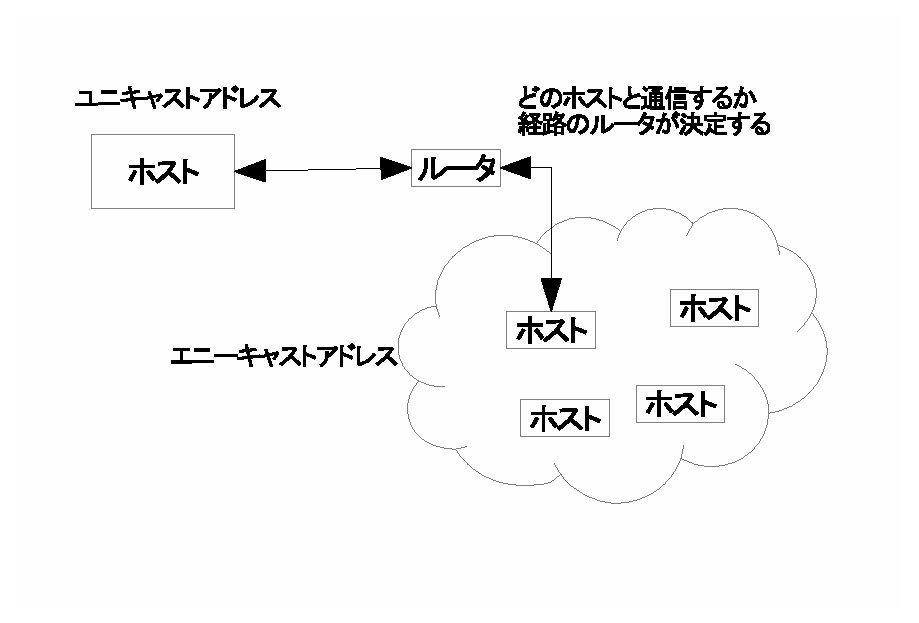
\includegraphics[width=12cm,clip]{draw/anycast.eps}
	\caption{エニーキャストアドレス}
	\label{fig:anycast}
\end{figure}

エニーキャストアドレスは、IPv6で追加されたアドレスである。

エニーキャストアドレスは、マルチキャストアドレスのように、あるネットワークの範囲で、ネットワークインタフェイスのグループを表す。だが、エニーキャストアドレス宛に送信したデータグラムは、そのグループに属するネットワークインタフェイスのどれかひとつが受信する。どのインタフェイスと通信するかは、経路の途中にあるルータが決定する。

エニーキャストでは最終的に一対一の通信となるため、宛先をエニーキャストアドレスとして、TCPを使用することもできる。だが、エニーキャストは通信相手が時間や状況の変化によって変わることがある。その場合、TCPのコネクションが切断され、新しい通信相手とハンドシェイクからやり直すことになってしまう。

そのため、データグラム型のUDPをトランスポート層のプロトコルとして使用することが多い。

エニーキャストアドレスは、たとえばネットワーク内のNTPやDNSサーバのように、最終的にネットワークに複数あるホストのどれが応えてもいい場合に使用する。たとえば、NTPサーバのグループにエニーキャストアドレスを付けておけば、NTP問い合わせに対して、エニーキャストアドレスを持ついずれかのホストが応答する。

\section{グローバルなアドレスとプライベートなアドレス}

ユニキャストのIPアドレスには、世界中でユニークであり、インターネット経由であるセス可能となるグローバルなアドレスと、プライベートなネットワークのみで使用するために範囲が設定された、プライベートなIPアドレスとに分けられる。

グローバル穴IPアドレスとプライベートなIPアドレスとは、用いるIPアドレスの範囲が異なる。

\subsection{ネットワークのスコープ}
あるネットワークの範囲という概念はどのようなものだろうか。それは、あるユニキャストアドレスやマルチキャストアドレスが、唯一のものとして判定される範囲ということである。これを、ネットワークのスコープとよぶ。

たとえば、LANの同じセグメントの中というスコープ、ルータで複数ネットワークが接続されたキャンパスネットワークの中というスコープ、インターネットで世界唯一として特定できるスコープ、などが考えられるだろう。

スコープは、たとえばルータが中継する、またはあるアドレス宛の通信を中継する、あるいは中継しないという判断の基準となる。

\subsection{IPv4のグローバルアドレス}
IPv4のグローバルなIPアドレスは、次に説明するプライベートアドレスの範囲、クラスD,クラスE、そして、特別なアドレスとして予約されている領域を除いた全てである。スコープという言葉を使えば、ワールドワイドなスコープである。

IPv4アドレスは元々、ARPA Netという、当時のグローバルなネットワークの中でユニークなインタフェイスを表すアドレスであった。プライベートアドレスの範囲などは、すべて後付けの概念である。

IPv4でグローバルなIPアドレスの割り当てを受ける際は、1つのインタフェイスに対して、ネットワークアドレスとホストアドレス全ての割り当てを受けるか、ネットワークに対して、ネットワークアドレス部分の割り当てを受けるかのどちらかになる。

前者は、割り当てられたひとつのインタフェイスのみが、グローバルなIPアドレスを持つ。後者は、ネットワークに対してネットワークアドレスを割り当てられるので、ホストアドレス部分は割り当てを受けた範囲で、任意に設定することができる。

\subsection{IPv4のプライベートアドレス}

IPv4アドレスには、外部に直接接続しないネットワーク(実験用、イントラネットなど)で、特に割り当てを受けなくても自由に使用できるIPアドレスの範囲が決まっている。このIPアドレスの範囲を、プライベートアドレスと呼んでいる。

プライベートアドレスのスコープを送信元とするデータグラムの宛先は、プライベートアドレスの割り当てられたホスト・ネットワークのみとなる。グローバルスコープのホストと直接通信することはない。

プライベートアドレスは、クラス毎に以下のように予約されている。

\begin{table}[hbtp] \caption{プライベートアドレスの範囲} \label{privateaddress}
\begin{center}
{\footnotesize
\begin{tabular}{lll} \toprule
クラス & ネットワークアドレス & アドレス範囲\\ \midrule
A & \verb+10/8+ & \verb+10.0.0.0-10.255.255.255+\\
B & \verb+172.16/12+ & \verb+172.16.0.0-172.31.255.255+\\
C & \verb+192.168.0/16-192.168.255/24+ & \verb+192.168.0.0-192.168.255.255+\\ \bottomrule
\end{tabular}
}
\end{center}
\end{table}

\subsection*{}
\begin{itembox}[l]{いもうとコラム IPv4のプライベートアドレスからのインターネットアクセス}
IPv4のプライベートスコープからグローバルスコープへ、直接の通信は行われません。でもこれは、通信をしてはならないという意味ではありません。

プライベートスコープのホストがグローバルスコープにアクセスする場合は、グローバルスコープのIPアドレスを用意し、そのアドレスを持つホストに、代わりにアクセスしてもらいます。プライベーツスコープのホストは、その結果をもらうことで、インターネットアクセスを行うわけです。

このように、アクセスを中継する役目を持つホストをプロキシといいます。プロキシにはアプリケーション層の代理アクセ宇を行うのプロキシ、トランスポート層の代理アクセスを行うNAPT(Network Address and Port Translation)もしくはIP masquarade、インターネットプロトコル層の代理アクセスを行うNAT(Network Address Translate)というようなものがあります。

\end{itembox}

\subsection{IPv6のグローバルアドレス}

\begin{figure}[htbp]
	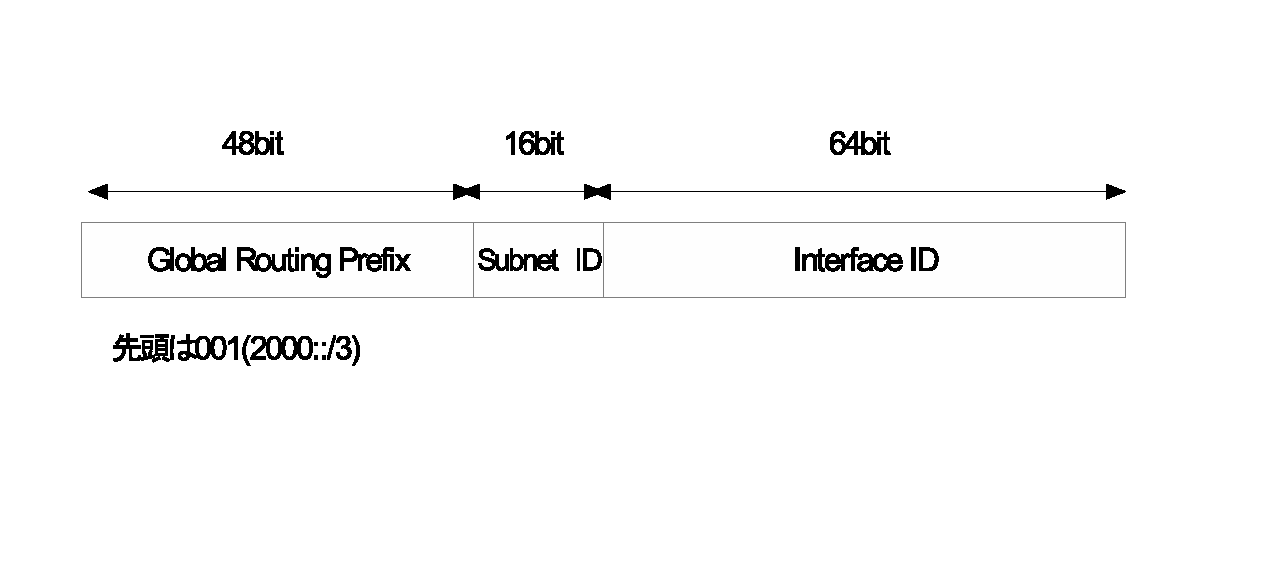
\includegraphics[width=12cm,clip]{draw/gua.eps}
	\caption{グローバルユニークアドレス}
	\label{fig:gua}
\end{figure}


IPv6によって世界で唯一のホストを特定するためのアドレスであり、発信元や宛先に指定したパケットが、インターネットに中継されるアドレスである。

先頭から48bit部分は、プロバイダによって割り当てられる。そのため、特に、グローバルプレフィクスとよんでいる。次の16bitはサブネットIDとよばれ、ユーザがサブネットを定義するために、任意に設定することが許される部分である。

だが、サービスによっては、プロバイダが、64ビットのプレフィックスを割り当ててくることがある。この場合、ユーザはサブネットを設定することはできない。

グローバルユニークアドレス発信元並びに宛先としたデータグラムは、全てのルータで中継を受けることができる。

\subsection*{}
\begin{itembox}[l]{いもうとコラム TLAとNLAとSLA}
古いIPv6の規格では、グローバルユニークアドレスは、TLA、NLA,SLAという部分による階層構造を取るというように定義されていました。。これは、インターネットサービスプロバイダ間でのアドレス割り当てが階層構造となることを想定したものでした。

ですが、現在は、グローバルプレフィクスとサブネットIDという、2段階の構造となっています。

\end{itembox}

\subsection{IPv6のリンクローカルアドレス}

\begin{figure}[htbp]
	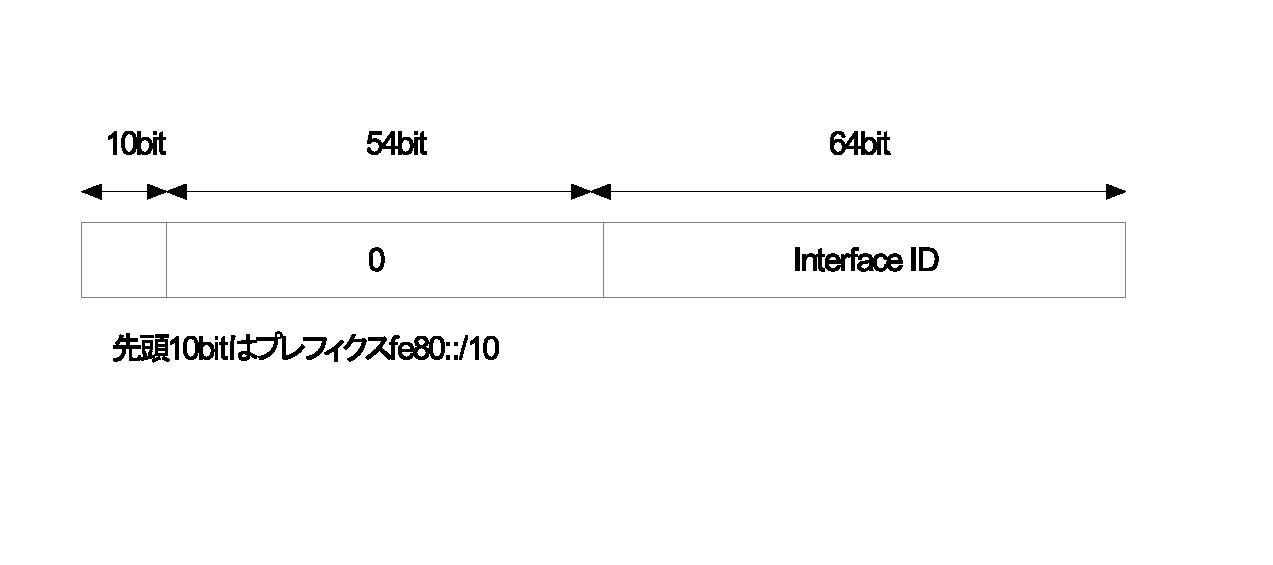
\includegraphics[width=12cm,clip]{draw/lla.eps}
	\caption{リンクローカルアドレス}
	\label{fig:lla}
\end{figure}

IPv6のリンクローカルアドレスは、ネットワークコミュニケーション層でいうところの、ひとつのネットワークをスコープとするアドレスである。つまり、リンクローカルスコープを用いた通信は、ルータで中継されることはない。そのため、リンクローカルアドレスには、サブネットIDのフィールドが存在しない。

リンクローカルアドr巣は、FE80::/10が割り当てられている。

また、リンクローカルアドレスを宛先に使用する場合、その通信の発信元のインタフェイスを併記する場合がある。

ここで気をつけなければならないのは、リンクローカルアドレスは、同一ネットワーク内での通信に使うためのアドレスであり、IPv4のプライベートスコープのアドレスにそうと酢売るものではないことである。


\subsection{IPv6のユニークローカルアドレス}

\begin{figure}[htbp]
	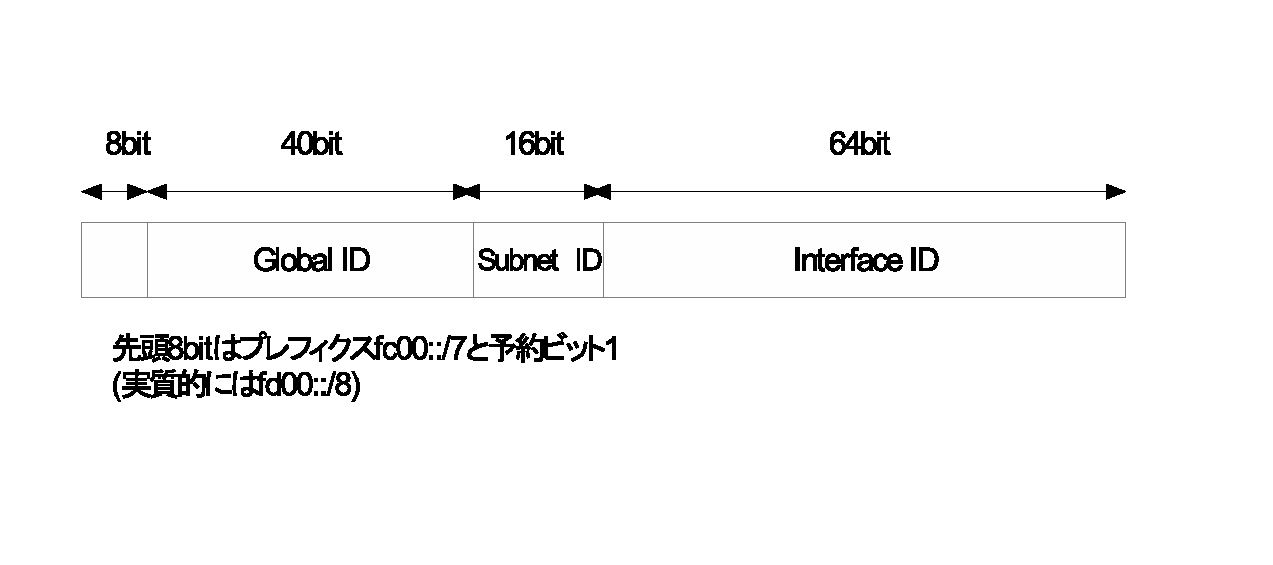
\includegraphics[width=12cm,clip]{draw/ula.eps}
	\caption{ユニークローカルアドレス}
	\label{fig:ula}
\end{figure}

IPv4にも、プライベートスコープアドレスがある。それが、ユニークローカルアドレスである。

元々はIPv6のアドレスは、グローバルユニークアドレスと、リンクローカルアドレスだけであった。あが、申請やプロバイダとの契約無しで、LANの中で使用可能なIPアドレスがあった方が便利であること、ネットワークインタフェイスにグローバルユニークアドレスを割り当てていると、ISPを変更することでプレフィクスが変更され、そのネットワーク内の機器全てで設定変更が必要になること、といった、実用面での理由から、ユニークローカルアドレスが制定された。

ユニークローカルアドレスは、グローバルIDと同様に、グローバルIDとサブネットID、インタフェイスIDから構成される。グローバルID部分は、fc00::/7が割り当てられ、この範囲で規定の手順でランダムに生成することが推奨されている。

インターネットに、ユニークローカルアドレスを宛先や発信元とするデータグラムを送出することはできない。だが、それ以外の、LAN内部のルータは、ユニークローカルアドレスを経由した通信を中継することができる。

\section{IPv6のマルチキャストアドレス}

\begin{figure}[htbp]
	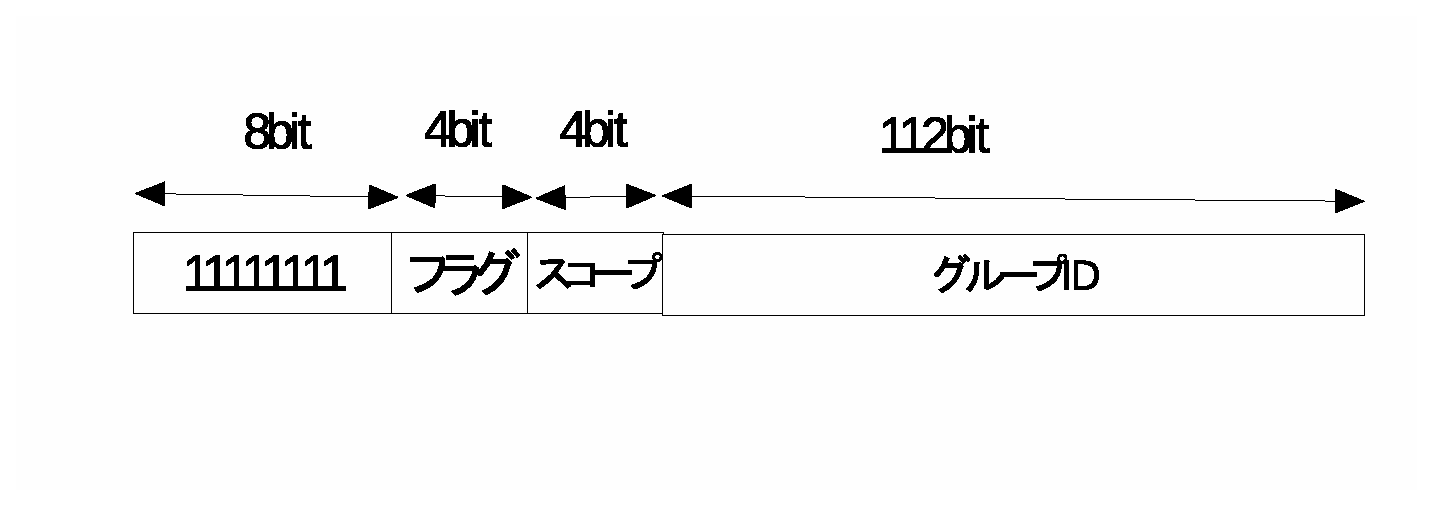
\includegraphics[width=12cm,clip]{draw/6multicast.eps}
	\caption{マルチキャストアドレス}
	\label{fig:6multicastaddr}
\end{figure}
マルチキャストアドレスは、ネットワークインタフェイスのグループを表すアドレスである。マルチキャストアドレスを宛先にしたデータグラムは、そのグループに属する全てのネットワークインタフェイスに届けられる。

IPv4ではオプションであったが、IPv6ではマルチキャストを積極的に利用する。ここでは、IPv6のマルチキャストについて、簡単に説明を行っていく。

マルチキャストアドレスは、おおまかに、プレフィクス部分と、グループID部分という構造を持つ。ユニキャストアドレスと違って、サブネットIDやインタフェイスIDはもたない。

また、マルチキャストアドレスでも、ユニキャストアドレスと同様に、スコープの考え方がある。これは、そのマルチキャストアドレスが存在できるネットワークの範囲が、スコープである。

IPv6のマルチキャストアドレスは、先頭8bitが必ず11111111、つまり、十六進数でFFとなる。次の4bitは、IANAによって割り当てられたアドレスであれば0、それ以外のテンポラリなものなら1を割り当てる。

スコープは4bitのフィールドで表される。このフィールドの数字は、そのまま、発信元のインタフェイスとルータを超えられる回数をイメージすれば良い。ノードローカルスコープは最大ホップ数が1なので、ホストが持つネットワークインタフェイスを越えられない。リンクローカルスコープは、最大ホップ数が2なので、ルータを越えることができない。そう考えれば何となくイメージできるだろう。

のこり112bitが、グループIDであり、あて先をあらわす。

だが、厳密には、インタフェイスローカル、リンクローカル、グローバルを除くスコープについては、管理者がIPv6ヘッダの最大ホップ数(ホップ制限)フィールドを適切に設定して、伝播範囲を制御する必要がある。

\subsection{インタフェースローカル}
インタフェースローカルスコープは、あるノード(ホスト)をスコープとする。古い資料ではノードローカルと記載されている場合がある。スコープのIDは1となる。

インタフェースローカルをいわば、マルチキャスト版のループバックアドレスである。では、どこがマルチキャストかのかというと、プロセスの待ち受けをグループ化する。

たとえば、スコープがインタフェースローカル、グループIDが101のNTPの場合、fe01::101は、自分自身の上で動いている全てのNTPサーバのプロセスが接続待ちしているポートを宛先とする。

また、ff00::1は、ノードローカルの全ノードが宛先であり、マルチキャスト版のループバックアドレスとなる。

\subsection{リンクローカル}
ルータ越えしない、同じネットワークの範囲でのマルチキャストである。スコープIDは2となる。

ff02:101は、ルータを越えずにアクセスできる全てのNTPサーバが宛先となる。
また、ff02::1であれば、ルータ越えしない、同じネットワークに接続されている全てのホストとなる。IPv4での、ブロードキャスト宛ての通信は、IPv6では、ff02::1を宛て諭したマルチキャスト通信となる。

IPv6が有効となっていれば、すべてのインタフェイスは、リンクローカルアドレスff02::1と、後ほど説明するNDP(Neiborhood Discovery Protocol(に用いられる要請ノードアドレスFF02::1:FF00:0000/104という二つのマルチキャストアドレスを持つ。要請ノードアドレス下位24bitは、ユニキャストIPv6アドレスのホストアドレス部分の下位3バイトとなる。


\subsection{組織ローカル}
組織ローカルスコープは、同一組織のネットワークをスコープとするマルチキャストアドレスである。スコープIDは8となる。

たとえば、同じ組織のネットワークにあるNTPサーバ全てにアクセスするなら、ff08::101が宛先となる。

組織ローカルスコープよりも範囲が狭い、サイトローカルスコープという概念もあるが、現在は推奨されないマルチキャストアドレスとされている。

\subsection{グローバル}
文字通り、インターネット全体をスコープとするマルチキャストアドレスである。だが、ヘッダで最大ホップ数が設定されるので、世界中に限りなく伝播していくわけではない。そうでないと、マルチキャストの転送ループが生じて、ネットワークが輻輳する。


\section{特別な意味を持IPアドレス}

IPアドレスに関した話題の最後に、特別な意味を持つユニキャストIPアドレスの説明を行なおう。これらのIPアドレスは、ネットワークやアプリケーションの設定でよく使用されるものである。

\subsection{デフォルトルートあるいは全ネットワーク}

IPv4で0.0.0.0/0もしくは、0.0.0.0/0.0.0.0と、IPv6で::、つまり全ビットを0として記述されるIPアドレスは、以下の二つの意味を持つ。

\begin{itemize}
\item デフォルトルート設定のときに、「自分と同じネットワークアドレスを持つIPアドレス以外のアドレス全て」を 表すアドレス
\item ネットワーク対応アプリケーションの設定などで、「全てのネットワーク」を表すアドレス
\end{itemize}

前者の意味で使用される場合は、ルートの設定がされていない宛先全て、という意味になる。また、後者の意味で使用されるときは、通信相手に関わらず同じ設定を適用したいときに用いられることが多い。

\subsection{ループバックアドレス}

IPv4で127/8もしくは127.0.0.0/8、IPv6で::1/128というように書かれる、クラスAのIPアドレスで、最大の番号を持つネットワークアドレスは、そのホスト自身を表すものとして予約されている。自ホストから送信された127/8宛のデータグラムは、ローカルループバックインタフェイスに送られる。

ローカルループバックは、便宜上127.0.0.1を使用することが多い。だが、ネットマスクを見て分かるとおり、127.0.0.0-127.255.255.255の、 16Mi個のIPアドレスが全て自分のローカルループバックインタフェイスを指す。実際、この範囲のどのIPアドレスに対して通信を行っても、ローカルループバックに到達するし、そのように実装しなければならない。

ループバックインタフェイスには、必ずループバックアドレスが割り当てられる。

\subsection*{}
\begin{itembox}[l]{いもうとコラム ループバックインタフェイスに割り当てるアドレス}
ループアバックインタフェイスには、必ずループバックアドレスを割り当てます。ですが、ループバックインタフェイスにはループバックアドレス以外を割り当ててることができます。

ループバックインタフェイスもネットワークコミュニケーション層のインタフェイスのひとつなので、ループバックインタフェイス以外のアドレスを割り当てることも可能です。
\end{itembox}


\subsection{リミテッドブロードキャストアドレス}

255.255.255.255は、IPv4アドレスのリミテッド・ブロードキャストアドレスと呼ばれる、特別なブロードキャストアドレスである。自分のIPアドレスが分からないネットワークインタフェイスが、そのネットワーク内にデータグラムを送信するときに使用する。例えば、IPアドレスをサーバから配布してもらうDHCPで、IPアドレスがまだ配布されていないクライアントが、DHCPサーバと最初の通信を行うのに使用する。

同じネットワーク(ネットワークコミュニケーション層のプロトコルで通信できるネットワーク)の全てのホストを宛先としてデータグラムを送信するために使用することは推奨されない。

IPv6では、このような場面ではマルチキャストアドレスを用いる。


\subsection{ドキュメント用アドレス}
IPv6に関するドキュメントを記述するためのアドレスとして、2001:db8::/32は予約されている。そのため、これをプレフィクスとして持つアドレスを発信元や宛先とするデータグラムを、インターネットに中継してはならない。







\section{データグラムとヘッダ}

ここまでで、インターネットプロトコルにおいて、バケツリレーのルールと、バケツリレーの宛先となるネットワークと、その中のホストを判別する方法を説明した。ここからは、バケツの中身、つまり、インターネットプロトコルでデータを送出する単位であるデータグラムを見ていくことにしよう。

インターネットプロトコル層では、データの単位を「データグラム」と呼ぶ。データグラムは、宛先のIPアドレス、送信元のIPアドレスなどの情報が記載されたヘッダと、宛先に届けるデータである、ペイロード部分から構成される。

ヘッダは、発信元IPアドレスと宛先IPアドレスを記入するフィールドとがある。TCP/IPのモデルで、IPアドレスを記載するのはIPヘッダだけである。

\subsection{IPv4ヘッダ}
IPv4のヘッダは、以下のような構造をしている。
オプションは必要に応じて追加し、32ビット境界になるようにパディングされる。そのため、ヘッダ部分は、20Byte以上で 4byte刻みの大きさとなる。

それぞれのフィールドの意味は、必要になった場面で説明しよう。
\begin{figure}
	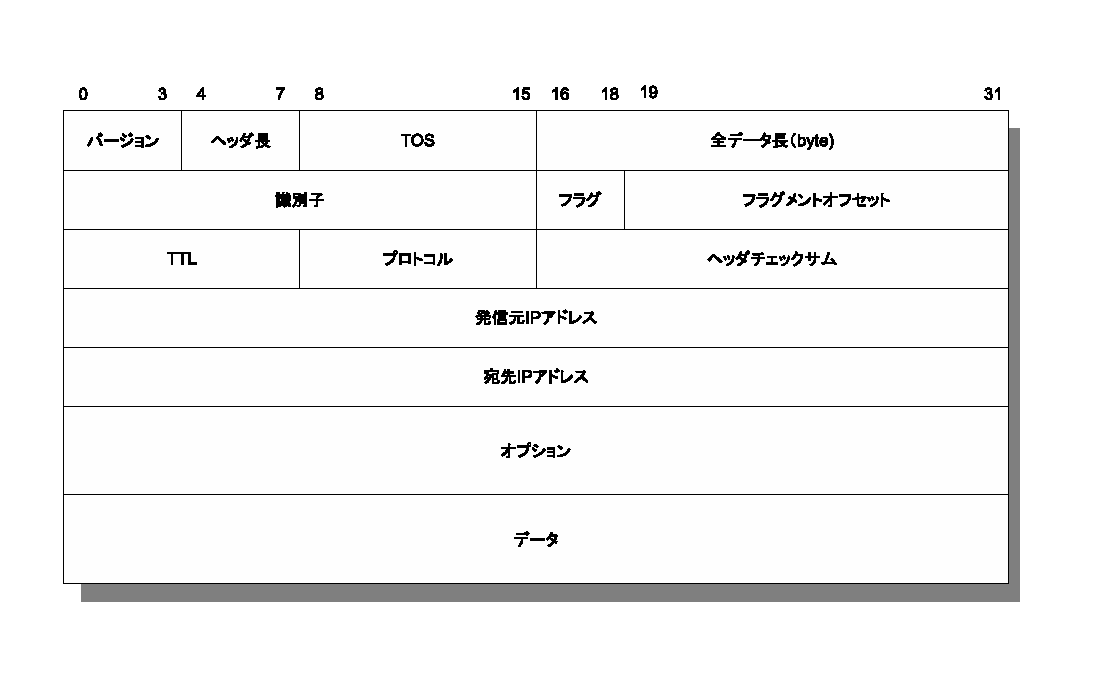
\includegraphics[width=14cm,clip]{draw/ipheader.eps}
	\caption{IPv4ヘッダ}
	\label{fig:ipheader}
\end{figure}

\subsection{IPv6ヘッダ}

\begin{figure}
	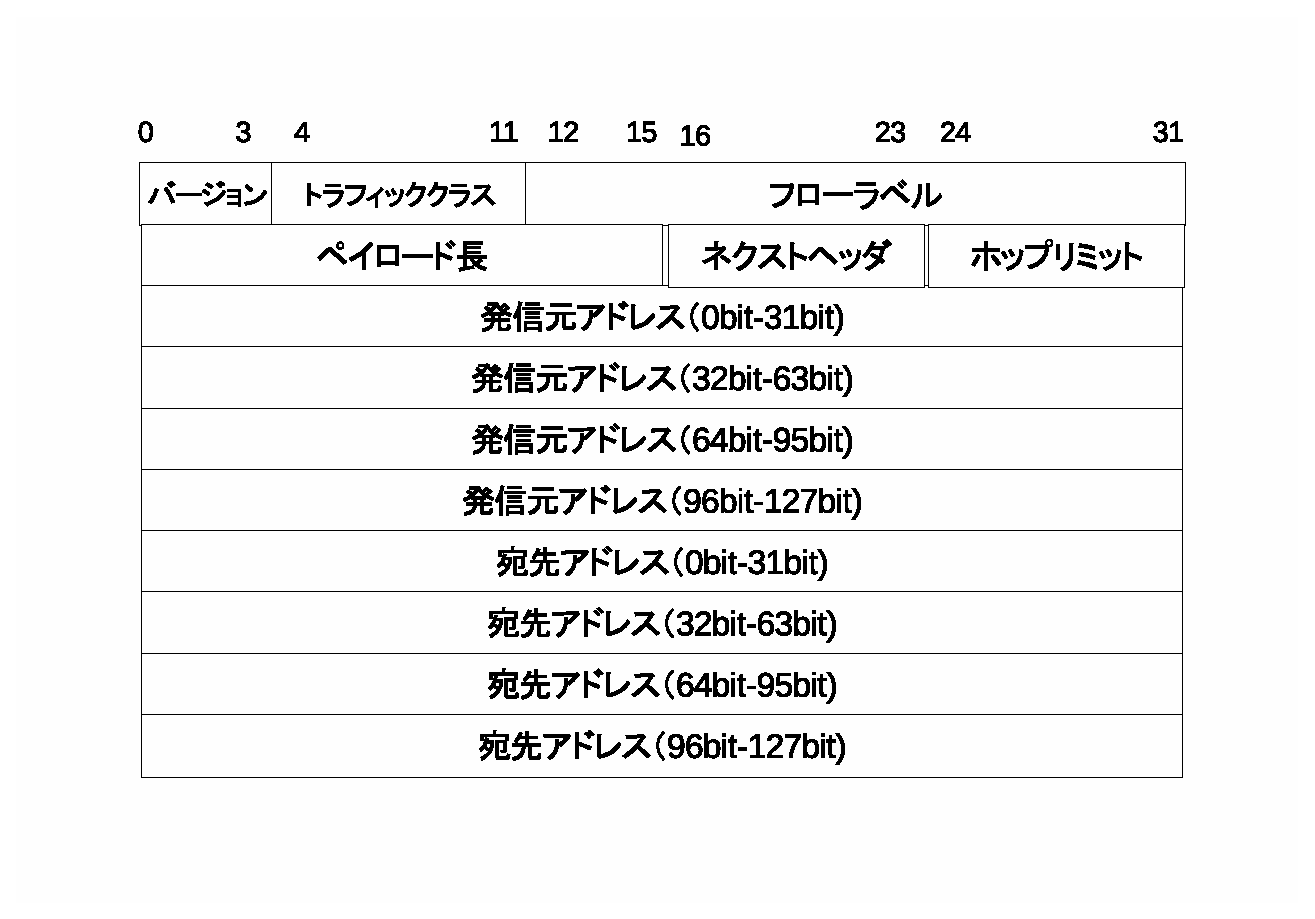
\includegraphics[width=14cm,clip]{draw/ipv6header.eps}
	\caption{IPv6ヘッダ}
	\label{fig:ipv6header}
\end{figure}

IPv6ヘッダは、図\ref{fig:ipv6header}ような構造をしている。チェックサムフィールドは、ネットワーク層やトランスポート層でデータの検査が行われることから、IPv6では省略された。それによって、サイズは大きいが構造はシンプルになっている。


\subsection{データグラムの最大の大きさ}
データグラムを実際に伝送するのは、ネットワーク内の通信を担当するネットワークコミュニケーション層である。そのため、ヘッダとデータからなるデータグラムのサイズの最大の大きさは、ネットワークコミュニケーション層の仕様に依存する。

また、ネットワークコミュニケーション層に依存しないデータグラムの最大サイズは、全データ長フィールドが16ビットなので、64Kibyteまでとなる。

IPv4では、全データ長フィールドは、ヘッダとデータの合計のサイズを入れる。そのため、実際に64Kibyteきっちりデータ部分にできるわけではない。

IPv6では、ペイロード長フィールドは、ヘッダを含まない、ペイロード部分のみの大きさとなる。これは、IPv6では、ルータ巻の転送によって、全てのヘッダの長さがかわることがあるためである。

\subsection{ネットワークバイトオーダと htonl()}

IPアドレスは、32ビット(4byte)を単位としたビット列としてネットワークコミュニケーション層に渡される。このときの送出順は、0ビット目(図\ref{fig:ipheader}の左側)から31ビット目(図\ref{fig:ipheader}の右側)にむけて「ビッグ・エンディアン」方向となる。これを、ネットワーク・バイトオーダという。

だが、x86系CPUなどは、24ビット~31ビット、16ビット~23ビット、8ビット~16ビット、0ビット~7ビットという、バイト単位で見たときにネットワークバイトオーダと逆順にメモリにコピーする仕様となっている。このような環境をリトル・エンディアンという。

そのため、プログラミングでIPアドレスを\verb+sockaddr_in+ 構造体にコピーする際に、\verb+htonl()+ という関数で、IPアドレスのビット列を、ネットワークバイトオーダで出力されるよう順番を入れ替えてから渡す。

一方、PowerPCやColdFireなど、ビッグエンディアンな環境では \verb+htonl()+ は不要なように思われる。だが、コードの移植性を考えて、常に\verb+htonl()+ を使用しておくようにする。\footnote{エンディアン変換の必要のない環境では\verb+htonl()+ は何もしないマクロとして定義されている。}


\subsection{IPv4ヘッダの最大・最小の大きさ}

データグラムのヘッダは、20byte以上の大きさで4byte(ワード長)刻みになる。では、そのヘッダの最大の大きさはいくつになるであろうか。

結論を言えば、最大の大きさは60byteとなる。これは、「ヘッダ長」フィールドが4bitであり、符号無しで最大値が15であることに由来する。ヘッダの大きさは、word(32bit、つまり4byte)単位で表される。

逆に、最小の大きさのヘッダは20byteとなる。この場合は5ワードになるため、ヘッダ長フィールドには5が記載される。

だが、実際のところ、IPヘッダのオプションフィールドが使用されることはほとんどない。IPv4ではヘッダ長フィールドがほとんど使用されなかったため、 IPv6では、IPヘッダを固定長として、ヘッダ長フィールドが廃止された。

\subsection{IPv6ヘッダの最大・最小の大きさ}
IPv6ヘッダは、サイズ固定である。その大きさは、40byteとなる。ただしこれは、ひとつのヘッダを可変長にしてオプション情報を詰め込むということをしない、という意味である。

IPv4では、可変長ヘッダが使われることはほとんどなかった。その知見から、IPv6ではヘッダの大きさは固定となっている。

\subsection{IPv6のネクストヘッダ}
\begin{figure}
	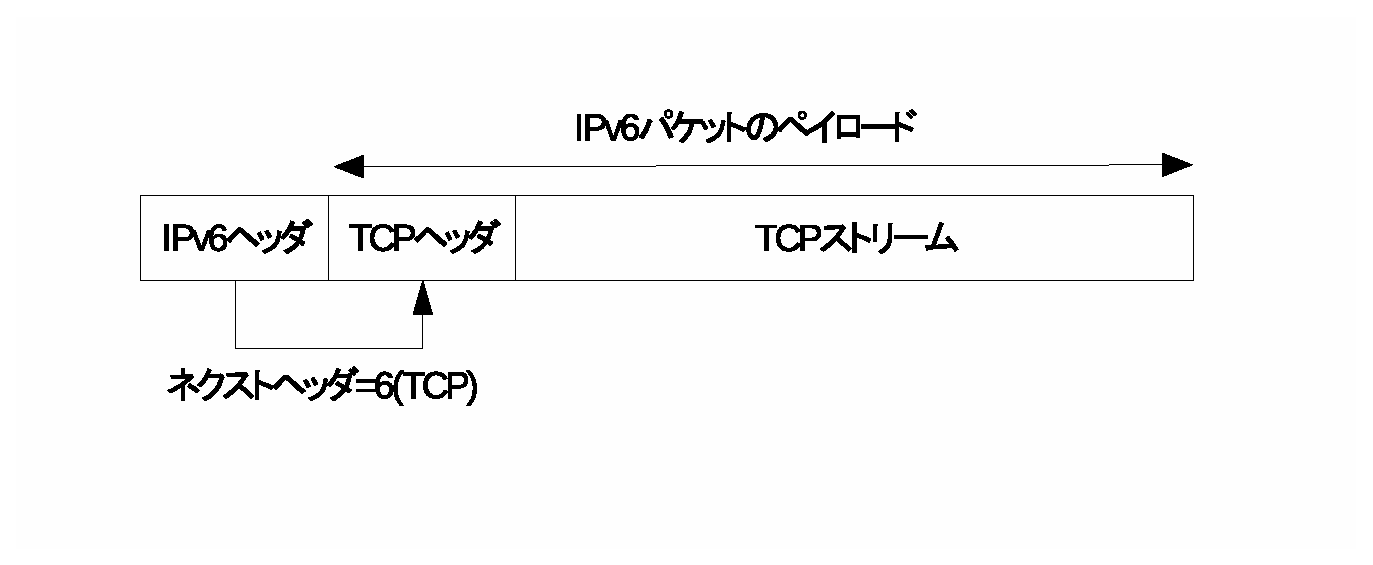
\includegraphics[width=14cm,clip]{draw/nextheader1.eps}
	\caption{IPv6のネクストヘッダ}
	\label{fig:ipv6nextheader}
\end{figure}

IPv6ヘッダには、ネクストヘッダというフィールドがある。これは、その名のとおり、IPv6ヘッダの跡に続く情報のヘッダがなにかをあらわすフィールドである。

では、ネクストヘッダフィールドは何に使われるのだろうか。このネクストヘッダは、IPv4のプロトコル番号フィールドとしての役割がある。ここにトランスポート層のプロトコルの番号を書けば、次のヘッダはトランスポート層のヘッダであり、ネクストヘッダ以降のペイロードをトランスポート層に渡す。

ここで、IPv6ヘッダの跡にトランスポート層のヘッダがくる、という点に注目しよう。インターネットプロトコル層のパケットの中では、IPv6ヘッダの後には必ず別のヘッダが来る。この概念を一般化すると、インターネットプロトコル層に関するオプションを、オプションヘッダという形で、ヘッダの後に続くヘッダとして定義する。それによって、各種オプションを一般化することができる。

この概念は、インターネットプロトコル層を中心にして考えたとき、複数のヘッダの後、上位層が運ぶべきデータがペイロードとして現れる、というものである。カプセル化の考えとも矛盾はしない。

では、オプションヘッダを使う例として、IPv6ジャンボデータグラムについて説明しよう。まず、インターネットプロトコル層は、IPv4,IPv6とも、ひとつのパケットの最大のサイズは64KiBである。これは、サイズのフィールドが16bitであるためである。

だが、IPv6ではジャンボデータグラムオプションという、それ以上の大きさのデータを転送するためのオプションがある。

IPv6のオプションヘッダには、ホップバイホップヘッダという、経路全てで参照されなければならないオプションヘッダがある。それに、ジャンボデータグラムの情報を付加して送信するわけだ。

ホップバイホップオプションをジャンボデータグラムのサイズ情報を格納するのに使用するとき、サイズ情報フィールドは、32bitとなる。このオプションを用いることで、最大4GiBの大きさのパケットを送信することが可能となる。

もうひとつ、IPsecのヘッダでも考えてみよう。IPsecのヘッダは、IPv4ではペイロード部分の先頭にあるビット列という考え方であったが、IPv6では、オプションヘッダのひとつとして、IPv6ヘッダの後に連結されるヘッダとなり、その後に暗号化されたペイロードが続く形となる。、

\begin{figure}
	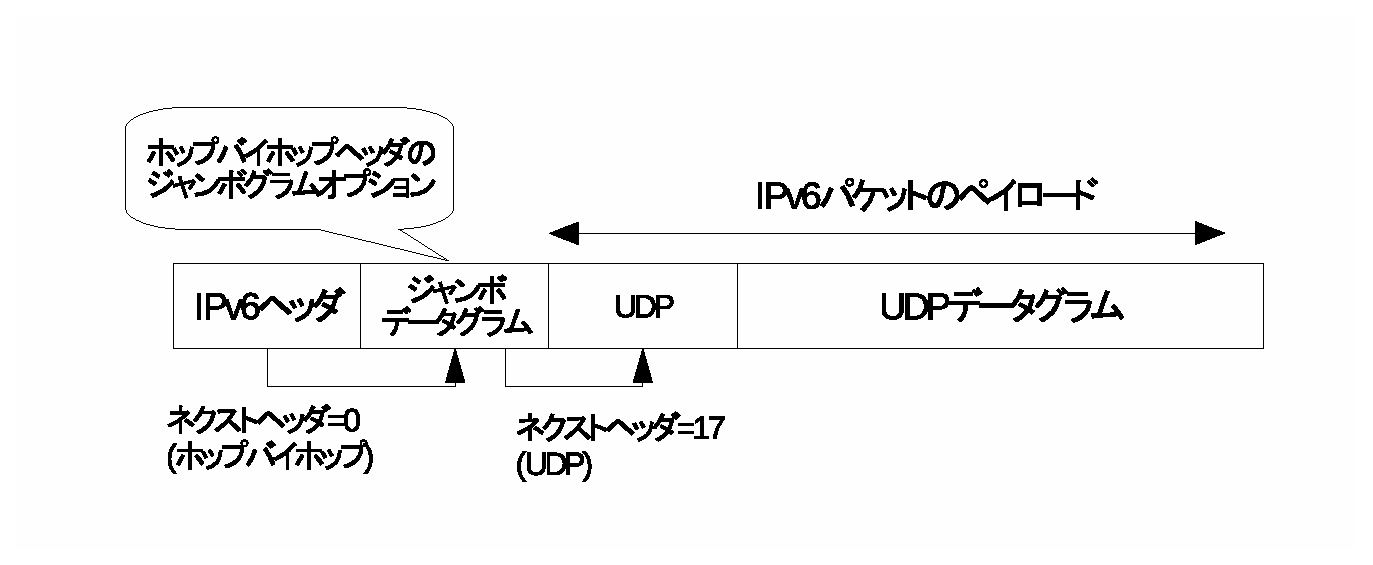
\includegraphics[width=14cm,clip]{draw/nextheader2.eps}
	\caption{IPv6のホップバイホップヘッダによるジャンボグラム}
	\label{fig:ipv6jumbogram}
\end{figure}


\subsection{ルータに中継してもらうデータグラムの宛先フィールド}

ルータに中継してもらうデータグラムのIPヘッダの宛先フィールドは、最終的に届けたいホストのIPアドレスとなる。間違えやすいが、ルータのIPアドレスではない。


では、そのデータグラムは、ヘッダにアドレスが書かれていないルータにどうやって届くのだろうか。ルータはネットワークコミュニケーション層のプロトコルで通信できる場所に接続されている。つまり、ネットワークコミュニケーション層のフレームの宛先が、ルータのネットワークインタフェイスとなるようにする。

インターネットプロトコル層では、自分宛でないデータグラムは、同じネットワークアドレス宛であれば、ネットワークコミュニケーション層を利用して、相手ホストにデータグラムを伝送する。別のネットワーク宛であれば、ネットワークコミュニケーション層を利用して、ルータにデータグラムを転送しようとするのは、ここまで説明したとおりである。

そして、インターネットプロトコル層レベルの通信は、その繰り返しで発信元からネットワークで接続された宛先に到着する。


\subsection{ルータに割り当てるIPアドレスに決まりはあるの?}
あるネットワークアドレスの範囲で、ルータ(デフォルトルート)に割り当てるホストアドレスをどれにするかという決まりはない。通常は、わかりやすくするために、そのホストアドレスの中でで一番小さい番号か、一番大きい番号かのどちらかから順番に割り当てることが多い

\section{IPv4の経路集約とCIDR}

IPv4では、ネットワークアドレスとホストアドレスをどこで分けるかの説明を思い出してほしい。先頭から8ビット目から30ビット目のどこかで分けると説明したときに、その方式の名前が CIDR(Classless Inter-Domain Routing)、であったことに違和感を感じなかっただろうか。

CIDRはその名の通り、元々は経路を集約する為に考えられたものであった。では、経路の集約とは何をすることだろうか。

たとえば、192.168.0.0/24のネットワークと192.168.1.0/24のネットワークが存在するとする。このとき、それぞれのネットワークが別々にに存在すれば、192.168.0.0./24に接続されたルータと、192.168.1.0/24に接続されたルータがそれぞれ必要になる。もちろん、経路も別々に記載し、設定しなければならない。

この例では二つのネットワークだけだから経路を全て記載してもたいしたことにならなかった。だが、これ世界規模になれば、経路を設定する手間が大変なことになる。そして、ルータが記憶すべき経路の量も大変なことになる。経路集約は、その負荷を減らす為の技術である。

ここまでの例でいくと、192.168.0.0/24と、192.168.1.0/24は、192.168.0.0/23というネットワークアドレスを持つネットワークの一部分、として扱う。つまり、外部から見たとき、192.168.0.0/24宛のデータグラムも、192.168.1.0 /24宛のデータグラムも、192.168.0.0/23というネットワークに接続されていることになっているルータに送ればいい。到着したデータグラムを、それぞれの宛先に応じて、どちらかのネットワークに転送するかは、最終的には192.1689.0.0/22のネットワークに接続されているルータの仕事となる。

では、なぜこういう方法をとることができるのだろうか。それは、IPヘッダのIPアドレスのフィールドには、ネットマスクの情報がないためである。つまり、データグラムがサブネットマスクの情報を持たないことを、恩恵として利用している。192.168.0.0/24及び 192.168.1.0/24以外のネットワークにあるホストは、このネットワークアドレスに対して送信するときに、これらのネットワークアドレスと 192.168.0.0/23を区別できない。

実際に、それぞれのネットマスクを適用したビットパターンで見てみよう。

\begin{table}[hbtp] \caption{ネットマスク23bitの場合} \label{mask23}
\begin{center}
{\footnotesize
\begin{tabular}{lll} \toprule
192.168.1.1/23 & バイナリ表記 & 十進表記\\ \midrule
ネットワークアドレス部 & \verb+11000000.10101000.00000000.00000000+ &192.168.000.000\\
ホストアアドレス部 & \verb+00000000.00000000.00000001.00000001+ & 000.000.001.001\\
IPアドレス & \verb+11000000.10101000.00000001.00000001+ & 192.168.001.001\\ \bottomrule
\end{tabular}
}
\end{center}
\end{table}

\begin{table}[hbtp] \caption{ネットマスク24bitの場合} \label{mask24}
\begin{center}
{\footnotesize
\begin{tabular}{lll} \toprule
192.168.1.1/24 & バイナリ表記 & 十進表記\\ \midrule
ネットワークアドレス部 & \verb+11000000.10101000.00000001.00000000+ & 192.168.001.000\\
ホストアアドレス部 & \verb+00000000.00000000.00000000.00000001+ & 000.000.000.001\\
IPアドレス & \verb+11000000.10101000.00000001.00000001+ & 192.168.001.00\\ \bottomrule
\end{tabular}
}
\end{center}
\end{table}

このように、ネットマスクの情報がなければ、この両社を区別する情報を、送信側が持つことはない。

\begin{figure}[htbp]
	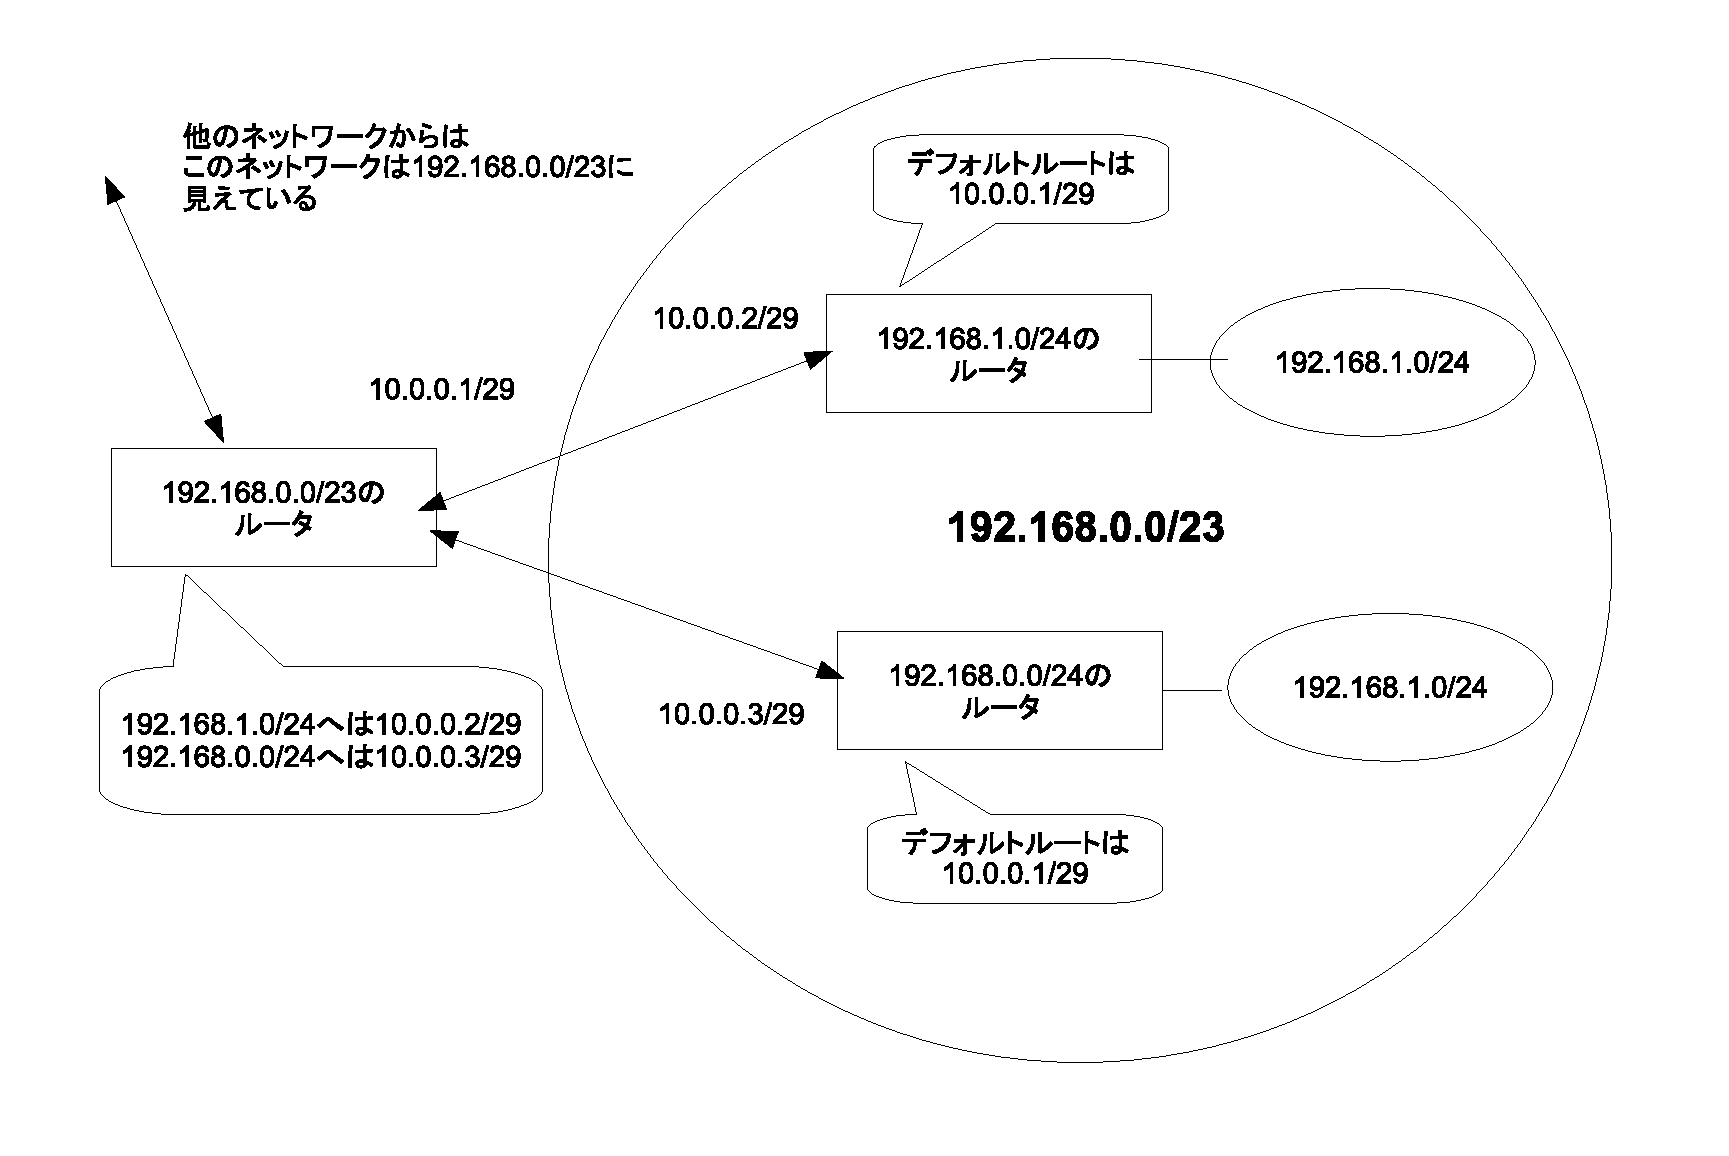
\includegraphics[width=12cm,clip]{draw/cidr.eps}
	\caption{経路集約}
	\label{fig:cidr}
\end{figure}

\subsection{サブネット}

\begin{figure}[htbp]
	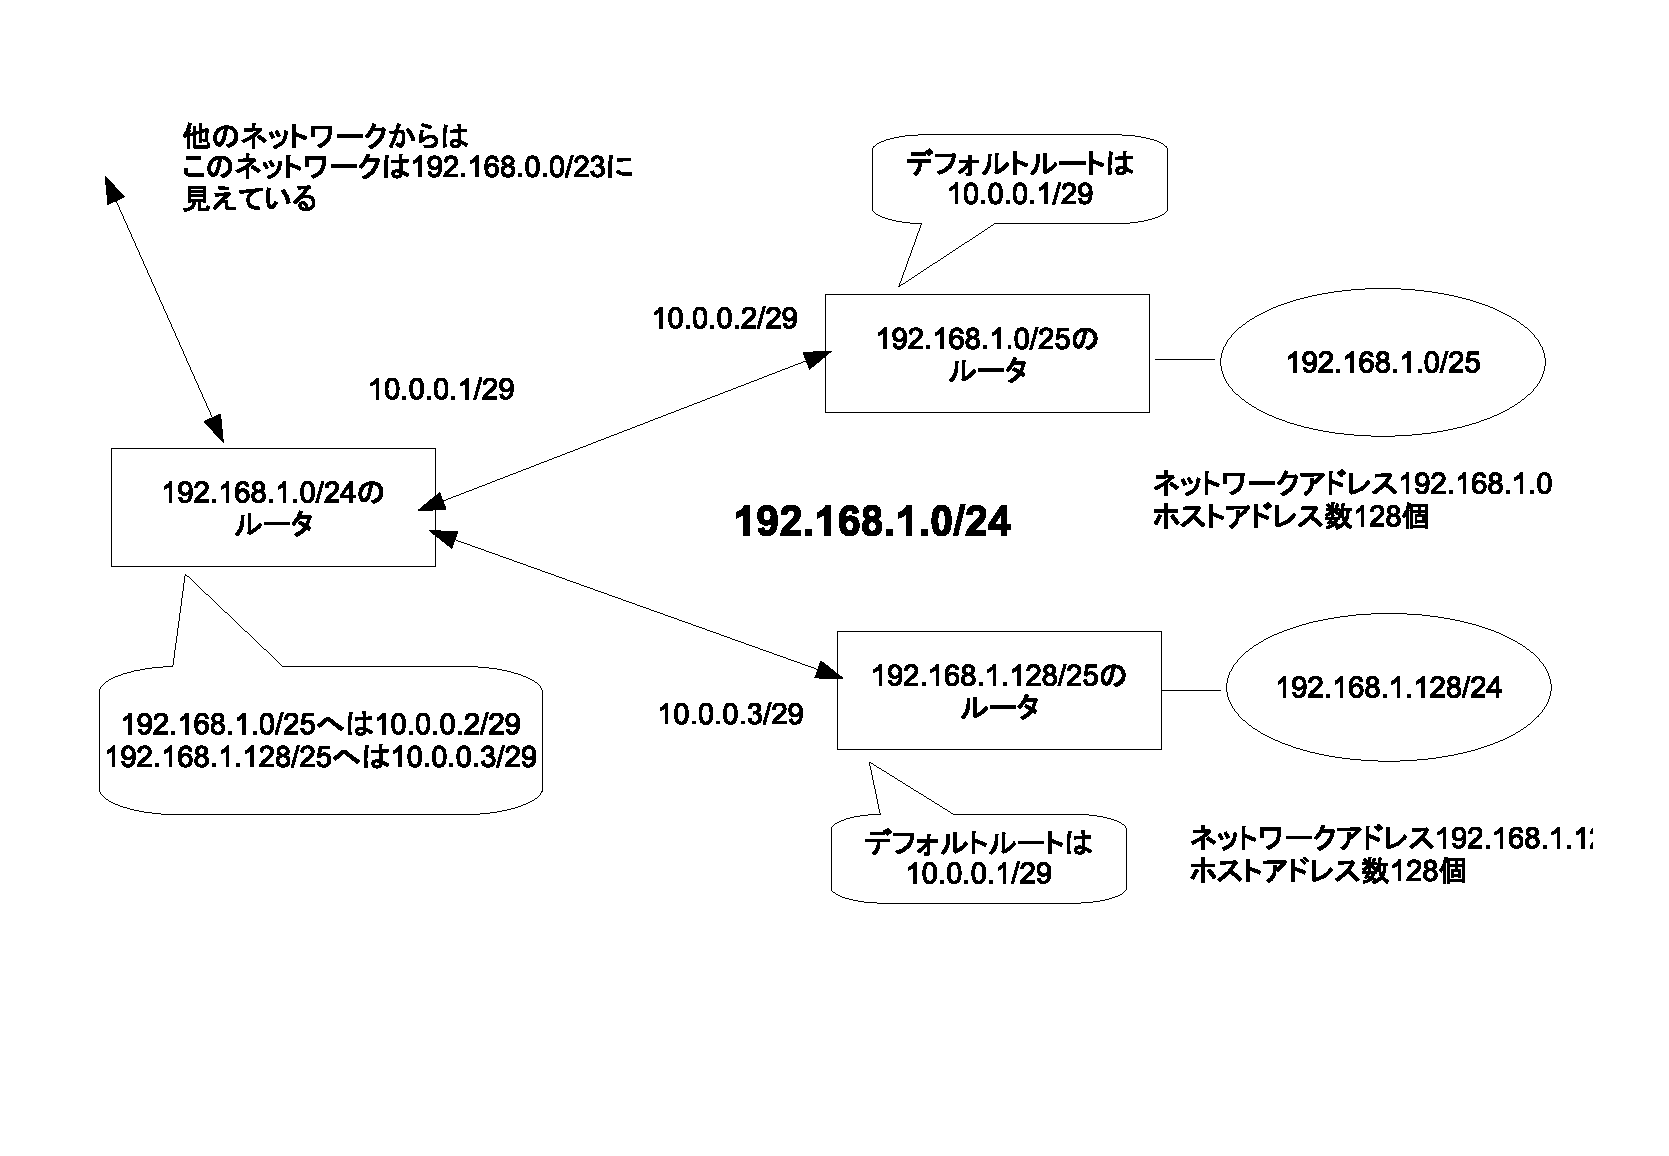
\includegraphics[width=12cm,clip]{draw/subbne.eps}
	\caption{サブネット分割}
	\label{fig:subnet}
\end{figure}

CIDRの考えを進めると、ホストアドレス$2^{n}$個のネットワークが作れると便利ではないか、という発想が出てくる。

たとえば、192.168.1.0/24という空間を16個に分割すると、ネットマスク28ビット、255.255.255.224となる。このネットマスクを192.168.1.0という,元のネットワークのネットワークアドレスに対して適用すると、192.168.1.0/28、 192.168.1.16/28,192.168.1.32/28…..192.168.1.224/28,192.168.1.240/28というネットワークアドレスを持つ、ホストアドレス16個の空間に分割することができる。

このように、元々のネットワークを、ネットマスクを変更することによって分割したネットワークを、サブネットという。また、サブネット分割を行うために変更したネットマスクを、サブネットマスクと言う。

この例では、外部のルータは、この16個のネットワークいずれかにアクセスする際は、192.168.1.0/24に接続されていることになっているルータと通信する。そうすることで、16個のネットワークのどれかに属する、 192.168.1.1,192.168.1.2……192.168.1.253,192.168.1.254というIPアドレス宛のデータグラム宛の通信は、問題なく行うことができる。

このように、任意の、$2^n$個のホストアドレス数を持つネットワークをつくることができれば、部署や組織の規模に応じたホストアドレス数を割り当て、結果、割り当てられたものの使用されずに死蔵されるIPアドレスを減らすことができる。

サブネットにも欠点がある。それは、分割されたサブネットの全てに、ホストアドレスのビット全て0(ネットワークアドレス)と、ホストアドレスのビット全て1(そのネットワーク内全てのホスト)が予約される。これにより、分割を行わない場合と比較すると、(分割数-1)×2個のIPアドレスをホストに割り当てることができなくなる。また、分割したネットワークから他のネットワーク(同じネットワークアドレスから分割した他のネットワークも含む)に対してデータグラムを送信しようとすると、そのネットワークが使用するためのルータ、もしくはデフォルトルートとなるルータが必要となる。

もう一つの欠点は、各ホストが、サブネットマスクを何らかの方法で認識しておく必要があるということである。ネットワークコミュニケーション層の機能を使って同じネットワーク内に送信すればよいかどうかの判断は、ネットワークアドレスを基準に行われる。IPアドレスからネットワークアドレスを取り出すためには、ネットマスクが何ビット目までかを知っておく必要がある。だが、ここまでで説明した歴史的経緯から、IPヘッダにはその情報を格納するフィールドがない。

ネットマスクの通知は、後に説明するICMPや、IPアドレスを自動設定するDHCPというプロトコルで、解決されている。

図\ref{fig:cidr}と図\ref{fig:subnet}を見比べればわかるように、経路集約とサブネット分割は同じ概念を言い換えただけである。このように、クラスレスのネットワークでは、経路を集約したり、大きなネットワークを分割して使ったりすることが可能である。

\subsection{IPv6の経路集約とサブネット分割}
IPv6では、アドレス体系の設計に、経路集約やCIDRの要素を含んでいる。IPv6のユニキャストアドレスのネットワークアドレス部は、48bitのネットワークそのものに部分と、サブネットを示す16bitのサブネットIDとからなる。経路集約を意識するときは、先頭48bitが同じネットワークをサブネットIDで分割する。

また、IPv6ではホストアドレスは56bitとすることが推奨されている。そのため。サブネット分割という考え方はない。もしサブネット分割的なことを行いたい場合は、ネットワークアドレスの末尾16bitを変こすることで、別のネットワークとする方法をとる。

\subsection*{}
\begin{itembox}[l]{いもうとコラム サブネット分割の歴史的経緯}
その昔、そこそこの規模の組織であれば、クラスBのIPアドレスをもらうことができた時代がありました。
ですが、IPv4アドレスの枯渇問題が明らかになったとき、一組織あたりに割り当てるホストアドレスの空間をCIDRによって減らすことで、当面の延命をはかったという経緯があります。

ナチュラルクラスでのIPアドレス割り当ては現在では珍しくなりましたが、近年ではソフトバンクグループがクラスAのアドレス空間の割り当てを受け、Interopが使用していたクラスAを返却しています。

\end{itembox}



\section{ICMP}
インターネットプロトコル層では、データグラムは投げっぱなしである。つまり、到着の確認や再送処理は、インターネットプロトコルの担当ではない。だが、それを送信元に対して通知する仕組みがあれば、上位のプロトコルが、データの再送を行うきっかけとしても利用することができるだろう。

その考えで規定されたのが、ICMP(Internet control Message Protocol)である。
ICMPは、インターネットプロトコル層が通信を制御するためのメッセージを、他のホストのインターネットプロトコル層に送信するためのプロトコルである。ICMPは、その伝送手段として、インターネットプロトコルを用いる。だが、インターネットプロトコル層はICMPを利用しない。

ICMPで得られたこの情報は、上位のプロトコルで利用することもできる。

ICMPはRFC792で定義されている。また、RFC950で、CIDRとサブネットに伴う拡張が追加された。また、IPv6で用いられるICMPの、ICMPv6は、RFC4443で定義された。

ここでは、単にICMPと書く場合はIPv4でのICMPを指し、IPv6でのICMPについては、ICMPv6と記載する。

\subsection{ICMPはどこにいるのか}

\begin{figure}[htbp]
	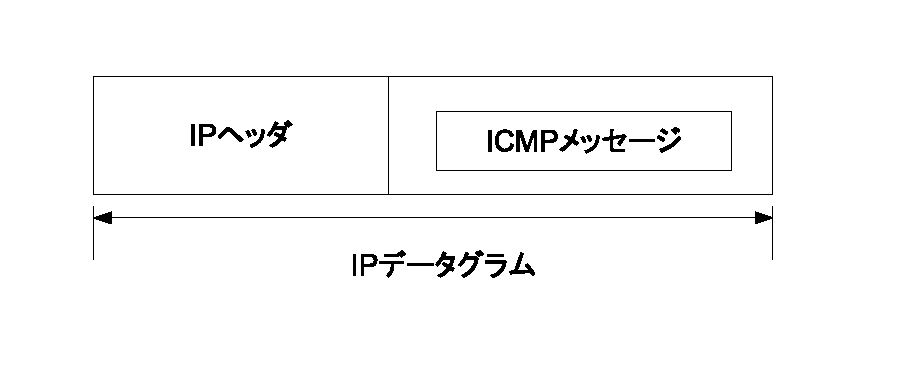
\includegraphics[width=12cm,clip]{draw/icmpencup.eps}
	\caption{ICMPデータグラム}
	\label{fig:icmpencup}
\end{figure}

ICMPは、インターネットプロトコルのパケットとして送信される。つまり、図\ref{fig:icmpencup}のように、IPデータグラムにカプセル化される。

ICMPは、レイヤーとしてはインターネットプロトコル層より上位にあるように見える。だが、アプリケーション層に通信路を提供するためのものではないので、トランスポート層ではない。だが、インターネットプロトコル層が自分では利用しないサービスであるため、居場所があいまいなところがあった。



RFC792のICMPの定義によると、ICMPは実装上はインターネットプロトコル層の上位プロトコルのように扱われる、実際にはICMPはインターネットプロトコルに不可欠の要素である。そして、全てのインターネットプロトコルのモジュールが実装しなければならない。

一方、ICMPv6は、トランスポート層より上への情報提供のみでなく、インターネットプロトコル層自身も利用する。そのため、インターネットpるとこる層の機能として考え易くなった。

\subsection{ICMPデータグラムの構造}

ICMPのデータグラムは、インターネットプロトコルのデータグラムが運搬するデータ、として送信される。ICMPメッセージの最初の4 バイトでのフィールドは共通で、それ以降のフィールドはメッセージによって異なる。そのため、ICMPはヘッダとデータ部分、という分け方はせず、全体をICMPメッセージとして扱う。

ICMPv6の場合、IPv6ヘッダのプロトコルフィールドに書き込まれるプロトコル番号は58となる。

図\ref{fig:icmpheader}で、タイプはメッセージのタイプ、コードは、メッセージのタイプ毎の伝達内容を表す。たとえば、コード3は宛先到達不可であり、タイプで、なぜ宛先に到達しなかったかを表す。

\begin{figure}[htbp]
	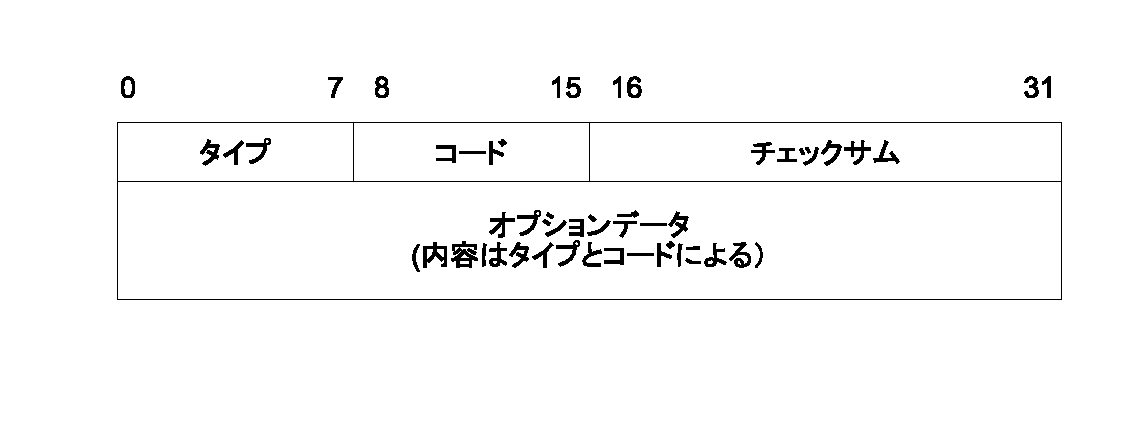
\includegraphics[width=12cm,clip]{draw/icmpheader.eps}
	\caption{ICMPデータグラムの構造}
	\label{fig:icmpheader}
\end{figure}


\subsection{ICMPで送信されるメッセージ}

ICMPでは、問い合わせとその応答、エラー発生時のメッセージが送信される。たとえば、PINGに使われるエコー要求とエコー応答、は、問い合わせとその応答である。また、何らかの原因でパケットが破棄された場合、その破棄したホストが送ってくるのメッセージは、エラーの通知である。

タイムスタンプや情報リクエストのように、通信のセッション管理に使用できるICMPメッセージもある。だが、この機能を使用したセッション管理は行なわれない。通信のセッション管理は、トランスポート層の機能を使用する。そして、それを実現するのが、次章で説明するTCPである。

ICMPによるメッセージの送信はmustではなくmayである。つまり、データグラムに対してICMPのメッセージ送信に該当する操作を行っても、送信の義務はない。そのため、セキュリティのために必要のない ICMPメッセージを返さないホストやルータも多い。

また、ICMPはパケットの受信の準備ができたことを相手に通知するものではない。あくまでも、データグラムが捨てられた事とその理由をインターネットプロトコル層レベルで通知するものである。そして、その通知が到達するかの保証はない。

\subsection{ICMPv6}
ICMPv6は、エラー情報を提供するもの、問い合わせと応答の機能がある。そして、IPv6で、ネットワークコミュニケーション層とIPv6アドレスのマッピングやアド絵レスの自動設定に用いる、近隣探索メッセージがある。

IPv6では、近隣探索メッセージをマルチキャストアドレス宛に送信し、各ホストからのその応答を取得する。または、その応答がないことを情報として利用する。
IPv6が有効なら、自動でかなr図設定されるマルチキャストアドレス宛に近隣探索メッセージを送信する。それによって、アドレスの自動割り当て、デフォルトルートの設定などが、IPv6の機能として実装されている。

\section{IPアドレスとネットワークコミュニケーション層のアドレスのマッピング}

インターネットプロトコル層のサービスには、同じネットワークに接続されあてょストとの通信も含まれる。そのとき、イーサネットなどのネットワークコミュニケーション層のサービスに対して通信相手を指定するために、IPアドレスとネットワークコミュニケーション層のアドレスのマッピングを行う必要がある。そのための情報収集の方法は、IPv4とIPv6とで異なる。

このマッピングによって、そのネットワーク内のホスト宛のパケットを乗せた、ネットワークコミュニケーション層のフレームを、どのホストに送信すればいいかを判断する。

ただし、PPPなど、一対一接続を行うためのネットワークコミュニケーション層であれば、ARPは行われない。なぜなら、ネットワークインタフェイスにお互いを区別するための名前がないためである。

ここでは、IPv4で用いるARPと、IPv6で用いるNDPとを比較することにしよう。

\subsection{NDPによるIPv6アドレスとMACアドレスのマッピング}
\begin{figure}[htbp]
	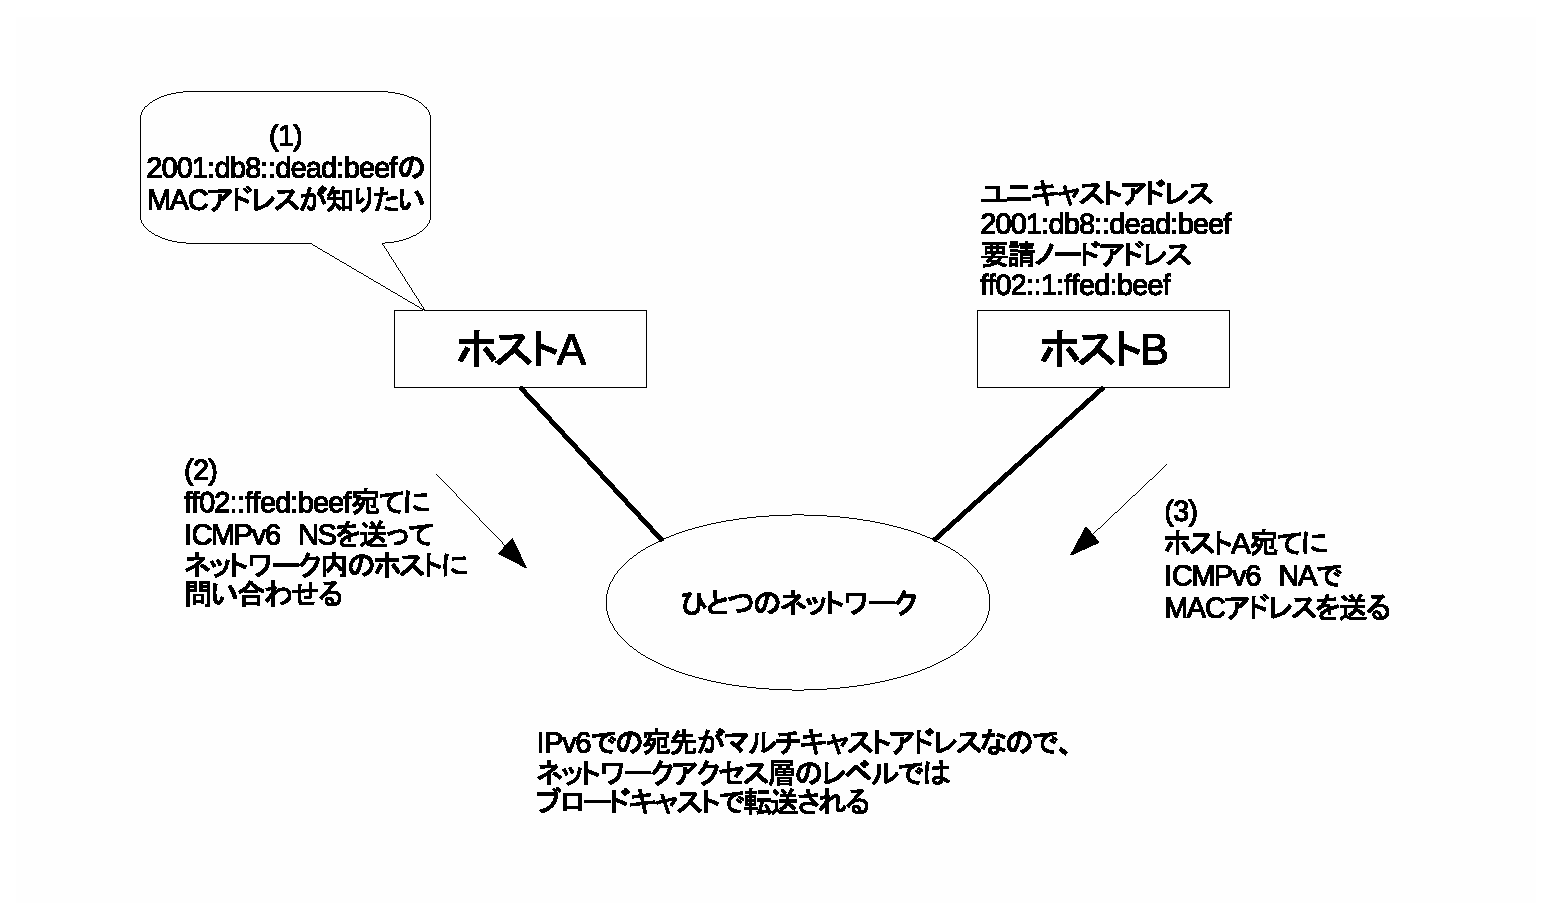
\includegraphics[width=12cm,clip]{draw/ndp.eps}
	\caption{NDPによるMACアドレス問いあわせ}
	\label{fig:NDP}
\end{figure}

ここでは、IPv6でIPv6アドレスとMACくぁドレスをマッピングするため情報収集である、NDPについて説明を行う。NDPは、Neighbor Disvocery Protocolで、近接探索プロトコルと呼ばれる。

近接探索には、ICMPv6を用いる。本稿では、その機能の一つである、IPアドレスとMACアドレスのマッピング情報の収集の説明を通じて、インターネットプロトコル層によるICMPv6の使用例を説明することを目的としたい。

NDP。IPv6アドレスやデフォルトルート情報の自動設定にも使われる。だが、本書は想定読者をネットワークアプリケーションを書くプログラマとしている。そのため、アドレス自動設定については割愛する。

前に、NDPで要請ノードアドレスを使用するという説明をした。要請ノードアドレスは、FF02::1::ff00:0000/104のマルチキャストアドレスで、下位3byteは、MACアドレスを調べたいIPv6ユニキャストアドレスのホストアドr巣部分の下位3byteと一致する。そのため、NDPを使いたい場合、ネットワークコミュニケーション層での同じネットワークに接続できるインタフェイスは最大4096となる。


\begin{enumerate}
\item 送信側は、IPアドレスに対応したMACアドレスを探す際、自分のメモリ上にある、IPアドレスとMACアドレスの対応表を調べる。この対応表を、キャッシュに格納する。キャッシュにIPアドレスとMACアドレスの対があればそれを利用して送信する。
\item キャッシュに情報がない場合、ICMPv6で、要請ノードアドレス宛に、ICMPv6のNS(Neihbor Solicitationを)
送信する。
\item あて先の要請ノードアドレスはマルチキャストアドレスなので、ネットワークアドレス層ではブロードキャストとして配送される。
\item ネットワーク内に、該当する要請ノードアドレスを持つホストがあれば、NSを受信する
\item NSのあて先となったホストは、ICMPv6のNA(Neighbor Advertisement)でMACアドレスを回答する。
\item 問い合わせ側はその結果を利用すると共に、一定時間キャッシュとして再利用する。
\end{enumerate}

このように、 ICPMb6を用いることで、MACアドレスの解決も、インターネットプロ取る層の機能だけで実現している。

\subsection{ARPによるIPv4アドレスとMACアドレスのマッピング}

IPv4の通信路として、イーサネットのような共用伝送媒体を使用するネットワークを使うとき、IPアドレスとネットワークコミュニケーション層のアドレスのマッピングはどのように行っているのだろうか。

それには、ARP(Address Resolution Protocol)というプロトコルを使用して、IPアドレスと物理的なホストの識別のマッピングを行う。このマッピングは、必要になったときに自動的に行われる。

以下、イーサネットにおけるARPの手順を説明する。イーサネット以外でも基本的な手順は同じである。

\begin{enumerate}
\item 送信側は、IPアドレスに対応したMACアドレスを探す際、自分のメモリ上にある、IPアドレスとMACアドレスの対応表を調べる。この対応表を、ARP テーブルと呼び、動的に生成される。ここにIPアドレスとMACアドレスの対があればそれを利用して送信する。
\item ARPテーブルに情報がない場合、ネットワークコミュニケーション層のプロトコルで、問い合わせを乗せたフレームをブロードキャストする。これをARP要求という。
\item ARP要求はブロードキャストで行われるので、同一ネットワーク内の全てのネットワークインタフェイスが受信する。もし、問い合わせに該当するIPアドレスが割り当てられているネットワークインタフェイスがあれば、それに応答する。これがARP応答である。
\item 問い合わせ側はその結果を利用すると共に、ARPテーブルに蓄積して、一定時間キャッシュとして利用する。
\end{enumerate}

ARPは、前述の通り、共有伝送媒体を使用する、つまり、ネットワークコミュニケーション層において、物理的なハードウエアを区別する手段があるネットワークに対して用いられる。PPPのように、ネットワークインタフェイスを一対一で接続するネットワークコミュニケーション層では、物理的なインタフェイスを区別する必要がない。そのため、ARPを用いる必要がない。

\begin{figure}[htbp]
	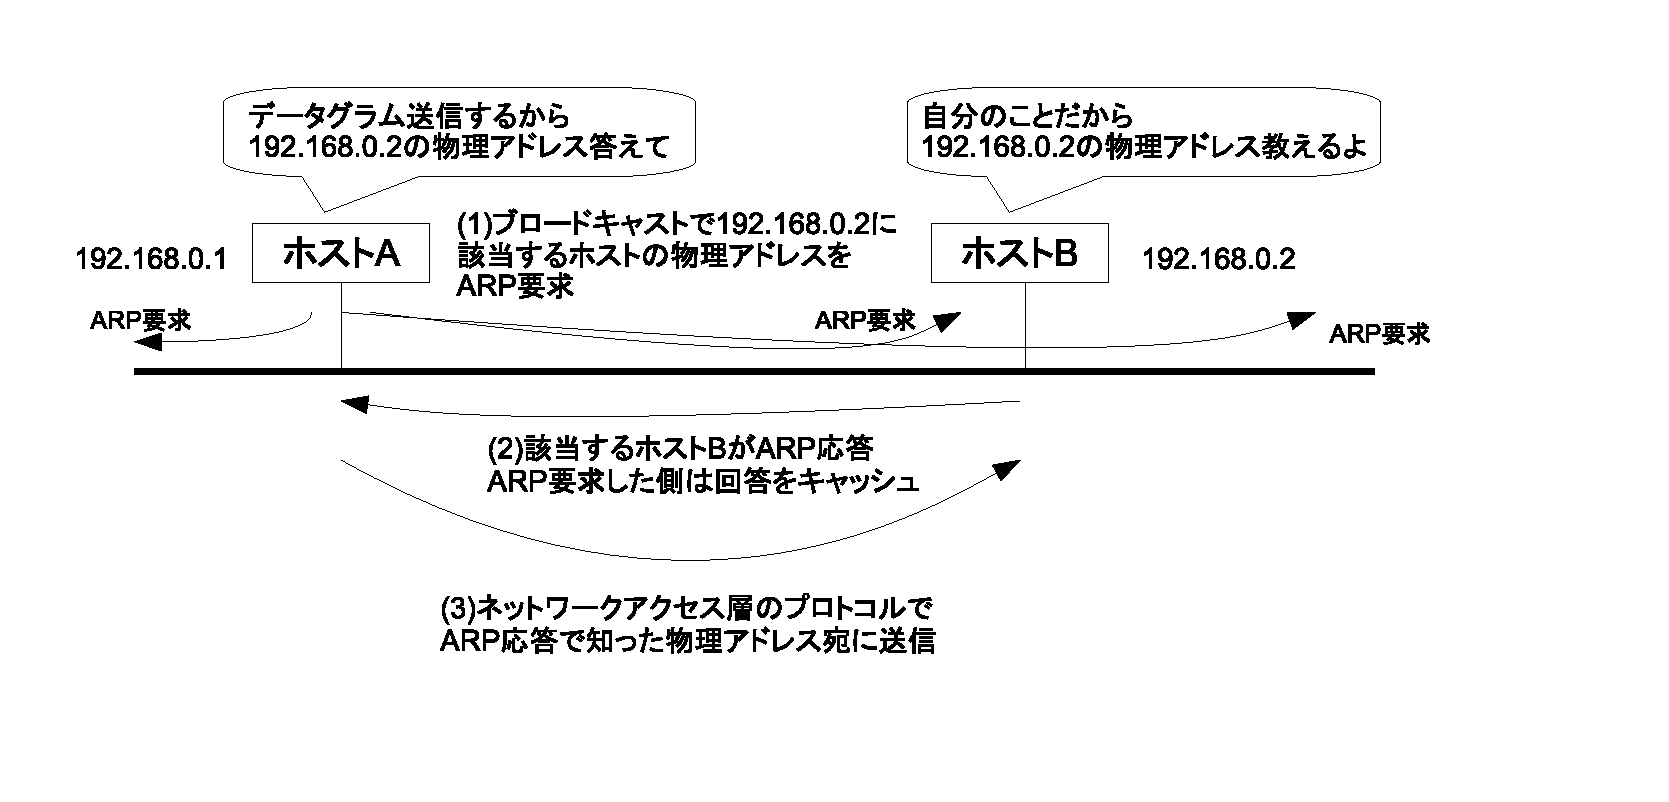
\includegraphics[width=12cm,clip]{draw/arp.eps}
	\caption{ARP要求とARP応答}
	\label{fig:arp}
\end{figure}

ここで、IPv6のNDPと、ARPを比較してみよう。ARP要求もARP応答も、IPv4はネットワークコミュニケーション層の情報を取得するのに、ネットワークコミュニケーション層のサービスを直接駆動している。通信路としてのサービス以上ことをネットワークコミュニケーション層に対して要求している。

後に現れたNDPのように、インターネットプロトコル層の機能で完結し、ネットワークコミュニケーション層はあくまでも経路としてのみ使うものとは本質的に異なる。だが、この知見が後のNDPにつながったと考えるべきであろう。


\section{パケットの寿命}

データグラムは、ネットワーク間を転送されることで、いつかは宛先にたどり着く。だが、途中のルータで転送先が間違っていたなどの理由で、宛先にたどり着かないまま転送され続ける、いわば迷子になったデータグラムも生ずる。

そのようなデータグラムは、どこかで消さないとネットワークのトラフィックを永久的に圧迫してしまう。そこで、IPv4ヘッダにはTTL(Time To Life)というフィールドを置いている。このTTLで、パケットがルータを通過できる残り回数をカウントする。

IPv6では、TTLでなくホップリミットというフィールド名となる。TTLが実際には時間でなくルータを通過した回数を数えるフィールドになったことから、わかりやすい名前に改められた。

パケットが送信されるとき、TTLもしくはホップリミットには、通常は64が設定される。この数値はルータを通過する毎に1ずつ減り、0になった時点でデータグラムは破棄される。これによって、迷子になったデータグラムがインターネットの上を回り続けることを回避している。

\subsection{寿命をわざと短くしたデータグラム}

HDDのビデオレコーダでは、LAN内に録画した番組を配信できるものがある。だが、この配信は、ルータを越えることができない実装が多い、つまり、インターネット経由でアクセスできないようになっている。これは、データグラムのTTLを1にすることで、そのビデオレコーダに一番近いルータがデータグラムを破棄するように細工がしてあるためである。

\section{フラグメントとゲートウェイ}

インターネットプロトコル層が、あるネットワークコミュニケーション層から上がってきたデータグラムを、他のネットワークコミュニケーション層に転送する場合を考えよう。

この二つのネットワークコミュニケーション層が同じ規格であれば、単純に、データグラムを転送先のネットワークのフレームにして送信すればよい。だが、転送先のネットワークコミュニケーション層の規格が異なる場合はどうであろうか。転送先のフレームのデータ部分が、最大サイズが現在のデータグラムよりも小さかった場合、インターネットプロトコル層では何をしなければならないか。

それは、転送先のネットワークコミュニケーション層のフレームに乗せることができるデータの大きさにあわせて、データグラムのサイズを変更することである。具体的には、データグラムの大きさが、転送先ののネットワークで扱えるデータの大きさになるように、データグラムのデータ部分を分割する。分割によって生じたデータクラムにも、新しくIPヘッダをつける。それによって、元が一つのデータグラムであったものを、よりサイズの小さい、複数のデータグラムとして送信し直す。

また、インターネットプロトコル層から見て、上位のプロトコルからストリームとして渡されたデータも、ネットワークコミュニケーション層で扱えるサイズになるよう分割し、その断片の全てにIPヘッダをつける。

この動作をフラグメントという。フラグメントするときのデータ量の単位となる、ネットワークコミュニケーション層におけるデータ部分のの大きさをMTU(Maximum Transmission Unit 最大転送単位)という。MTUは、ネットワークコミュニケーション層のフレームの大きさではないことに注意してほしい。

インターネットプロトコル層は、ヘッダとデータの断片一つの大きさを合計したものがMTU以下になるよう、データを分割する役目ももっている。

このように、異なるMTUを持つ、つまりネットワークコミュニケーション層の構成・構造が異なるネットワークの間で中継を行うIP層の機器を、ルータと区別してゲートウェイト呼ぶことがある。

IPv6では、経路のMTUは、ICMPv6を用いて調べることができるようになった。この手順を、PMTUや、Path MTU Discoveryと呼ぶ。PMTUは、RFC1191で定義されている。

\subsection{フラグメントのタイミング}
インターネットプロトコル層のフラグメントは、どのタイミングで行われるのだろうか。これ派、IPv4とIPv6とで、行うことが許されるタイミングが異なる。

IPv4では、あるルータが、直接転送する先への送信でフラグメントが必要であれば、フラグメントを行って送信する。これは、パケットを中継するすべてのルータが、必要であればフラグメントを行う、といことである。MTUは、直接転送する先のルータまでの経路で図られる。

一方のIPv6は、インターネットプロトコル層ではフラグメントを行わない。もし、直接通信するルータまでの経路のMTUよりも大きなパケットが到着したら、それを破棄してICMPv6で通知する。


通信の始点だけが、フラグメントを行う。送信の前にあて先までの経路のMTUを調べ、それにあわせて送信する。これは、現代では、インターネット接続に使われる経路が、パケットの転送中にかわる、つまりパケット転送中に、経路のMTUが変化することはほぼないことから、実装をシンプルにするための仕様である。

そのため、IPv6は、最初に、経路ののPMTUディスカバリを実行し、経路の最小MTUサイズを求める。そして、途中でフラグメントが必要ないMTUを設定し、データを送信する。また、フラグメントが発生した場合は、ネクストヘッダ番号41のIPv6-Fragヘッダを付加して、それぞれのフラグメントを送信する。受信側は、そのフラグメントヘッダの情報から、元のデータグラムを再構築する。


\subsection{中継先のネットワークのMTUの方が大きいときは?}

インターネットプロトコル層が、データグラムの大きさよりもMTUの小さいネットワークにデータを転送するときはフラグメント処理を行う。では、転送する先のネットワークコミュニケーション層のMTUが、フラグメントした後のデータグラムよりも大きい場合はどうするのだろうか。

この場合はなにもしない。つまり、フラグメントを収集してデータグラムを再構築する、という処理は行われない。。理由としては、フラグメントの再構築を行うには、分割された全てのデータグラムを収集する必要がある。だが、ここまでで説明した通り、インターネットプロトコル層の性質として、全てのフラグメントが再構築を行おうとするインターネットプロトコル層を経由する保証がないことを思い出してほしい。

そのため、インターネットプロトコル層は、転送先となるネットワークコミュニケーション層のMTUが、現在のデータグラムのサイズより小さいときのフラグメント処理しか行わない。

\subsection{フラグメントされたデータの再構築}

自分が宛先であるデータグラムを受信したときに、インターネットプロトコル層は、元のデータを構成するフラグメントを全て蓄積し、データを再構築して、ストリームとして上位プロトコルに渡す。もしこのフラグメントが一定時間内にそろわなければ、タイムアウトとして、収集したフラグメントを全て破棄する。

フラグメントされたデータを元のストリームに戻すために、インターネットプロトコル層は、IPヘッダの識別子と、フラグメントオフセットのフィールドに記載された情報を用いる。

断片がそろわずにデータグラムが破棄された場合、インターネットプロトコル層は発信元にフラグメント破棄の通知を行わない。これはデータグラム破棄の通知として、ICMPを用いて行われる。

\subsection*{}
\begin{itembox}[l]{いもうとコラム インターネット物理モデル}


実は、インターネットプロトコルの動作を見ることができる場所があります。お台場\footnote{実際の住所は江東区青海 http://www.miraikan.jst.go.jp/}にある日本科学未来館に、インターネット物理モデルという、IP層まの動作を再現したモデルが展示されています。

インターネット物理モデルは、白と黒のボールをビットとして使用し、それを端末である操作台の溝の上にならべます。それによって宛先IPアドレスとデータからなるパケットができるわけです。

次に、送信レバー(!)を引くと、パケットである、一列に並べられたボールがルータに送り込まれます。

そのルータはボールの列のヘッダであるIPアドレスを識別して、宛先となる端末と繋がっているルータに送り込みます。そして、IPアドレスに対応する宛先がない場合は、そのデータグラムはエクスパイアされます。早く言えば、ルータの下にあるかごにボールが捨てられるわけです。

図\ref{fig:miraikan}は、インターネット物理モデルの写真でする。左側にあるのが操作台で、右側の機械(ルータ)と、レールで接続されています。
\end{itembox}


\begin{figure}[htbp]
	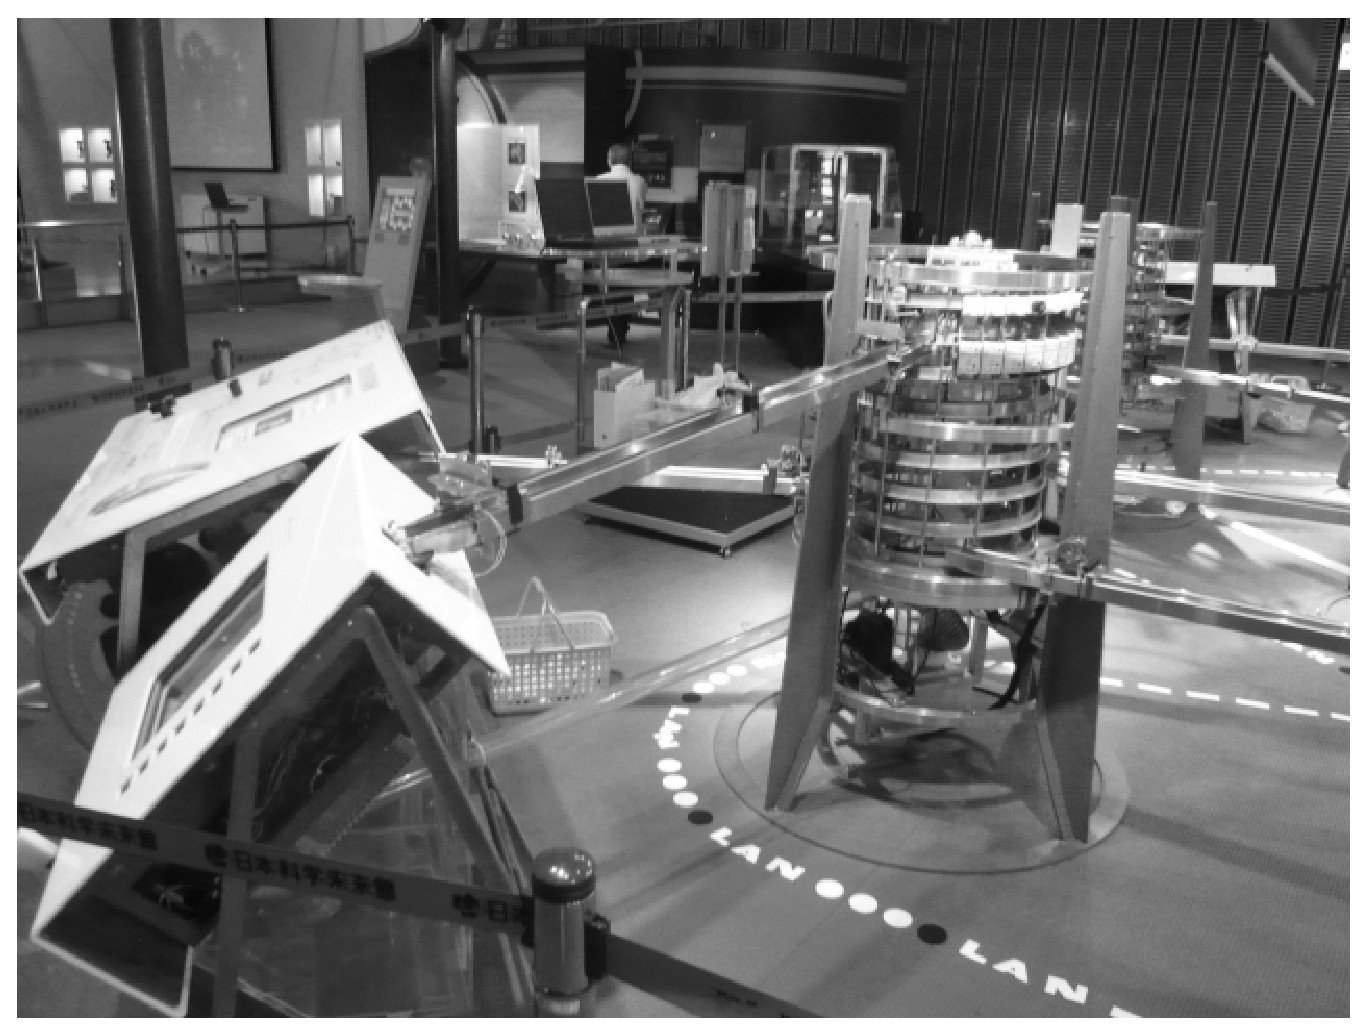
\includegraphics[width=12cm,clip]{draw/miraikan.eps}
	\caption{インターネット物理モデル}
	\label{fig:miraikan}
\end{figure}

